\documentclass[11pt,a4paper,ngerman]{article}
\usepackage[ngerman]{babel}% deutsche Trennregeln
\usepackage[T1]{fontenc}% wichtig f�r Trennung von W�rtern mit Umlauten
\usepackage{microtype}% verbesserter Randausgleich
\usepackage[latin1]{inputenc} 
\usepackage{babel}
\usepackage{ae}
\usepackage{bchart}
\usepackage{float}
\usepackage{ulem}
\usepackage{tikz}
\usepackage{mathpazo}
\usepackage{pgfplots}
    \pgfplotsset{compat=newest}

\usepgfplotslibrary{statistics}
\usetikzlibrary{arrows,shapes,positioning,shadows,trees,er}
%tikz-setup for drawing trees
\tikzset{
  basic/.style  = {draw, text width=2cm, drop shadow, font=\sffamily, rectangle},
  root/.style   = {basic, rounded corners=6pt, thin,align=center, fill=green!60,
                   text width=8em},
  level 2/.style = {basic, rounded corners=6pt, thin,align=center, fill=green!60,
                   text width=8em},
  level 3/.style = {basic, thin, align=left, fill=pink!60, text width=6.5em}
}
%
%
%
\usepackage{fancyref}
\usepackage{fancyhdr} 
\usepackage{xcolor}
\usepackage{framed}
\usepackage{url}
\usepackage{makeidx}
\usepackage{colortbl}
\makeindex
\usepackage{listings}

%
%Colors
\definecolor{shadecolor}{rgb}{0.9,0.9,0.9}
\definecolor{skyblue}{rgb}{0.447,0.624,0.812}

% PDF settings
\usepackage[pdfstartview=FitH,pdftitle={Messung der Informationstypen-H�ufigkeiten in der Python-Dokumentation },pdfauthor={Sven Wildermann}, colorlinks=false, linktocpage, pdfborder={0 0 0 }]{hyperref}
% colorlinks=false, pdfborder={0 0 0} = keine farbigen Links
%
 %
% Header and Footer Style
\pagestyle{fancy}
\fancyhead{}
\fancyhead[R]{\slshape Sven Wildermann}
\fancyhead[L]{\slshape\nouppercase{\rightmark}}
\fancyfoot{}
\fancyfoot[C]{\thepage}
\renewcommand{\headrulewidth}{0pt}
\renewcommand{\sectionmark}[1]{\markright{\thesection\ #1}} 
%
% No identation
\setlength\headheight{15pt}
\setlength\parindent{0pt} 
%
% Custom commands
\newcommand\zb{z.\,B.\ }
\renewcommand\dh{d.\,h.\ }
\newcommand\parbig{\par\bigskip}
\newcommand\parmed{\par\medskip}
\newcommand{\mailto}[1]{\href{mailto:#1}{#1}}
%
% Python Code Listing Style
\definecolor{skyblue}{rgb}{0.447,0.624,0.812}
\definecolor{darkblue}{rgb}{0,0,.6}
\definecolor{darkgreen}{rgb}{0,0.5,0}
\definecolor{darkred}{rgb}{0.5,0,0}
\lstset{language=Python, basicstyle=\ttfamily\small\upshape, commentstyle=\color{darkgreen}\sffamily, keywordstyle=\color{darkblue}\rmfamily\bfseries, breaklines=true,tabsize=2,xleftmargin=0mm, xrightmargin=0mm,numbers=none,frame=single,stringstyle=\color{darkred},
showstringspaces=false,numbers=left,frame=none}
%
% Titel and author 
\title{
\includegraphics[width=0.6\textwidth]{pictures/logo}\\
{\normalsize Bachelorarbeit am Institut f�r Informatik der Freien Universit�t Berlin, Arbeitsgruppe Software Engineering}\\[6ex]
Messung der Informationstypen-H�ufigkeiten in der Python-Dokumentation}

\author{Sven Wildermann\\
{\normalsize Matrikelnummer: 4567553}\\
{\normalsize \mailto{bachelorarbeit@wildermann.berlin}}\\\\
{\normalsize Betreuer und Gutachter:  Prof. Dr. Lutz Prechelt}\\
{\normalsize Zweitgutachterin: Prof. Dr. Elfriede Fehr }}

\date{Berlin, 12. August 2014}


\begin{document}

\begin{titlepage}


\pagenumbering{alph}
\maketitle
\thispagestyle{empty}

\vfill{}
\vfill{}

\end{titlepage}

\pagestyle{empty}
\clearpage\pagenumbering{roman}

%\newpage
%\thispagestyle{empty}
%\mbox{}

\section*{Zusammenfassung}
Walid Maalej und Martin P. Robillard haben im September 2013 einen Artikel \cite{MaalejRobillard} ver�ffentlicht, in dem sie die Dokumentationen der Programmiersprachen Java und .NET auf ihren Informationsgehalt hin untersucht und verglichen haben. Diese Untersuchung wird im Rahmen dieser Bachelorarbeit auf die Dokumentation von \href{https://www.python.org/}{Python}\footnote{https://www.python.org/} mit einigen Abweichungen �bertragen. \\
Die von Maalej und Robillard eingef�hrte Taxonomie der in Dokumentationen anzutreffenden Wissenstypen wurde hierf�r auf die Eigenheiten von Python angepasst. Die Einordnung von Teilen der Dokumentationen zu den verschiedenen Wissenstypen wird von Gutachtern im Rahmen eines Forschungspraktikums geleistet und erfolgt mit Hilfe eines eigens hierf�r geschriebenen Werkzeuges. \\
Die anschlie�ende Auswertung der Ergebnisse und Vergleich dieser mit denen aus dem Originalartikel zeigt, dass die vorgenommenen �nderungen in der Konzeption sinnvoll waren und f�r noch eindeutigere Ergebnisse gesorgt haben. Die Struktur der Wissenstypen in der Dokumentation von Python �hnelt stark der bei Java und .NET gefundenen, hat aber auch �berraschende Abweichungen. Die erhobenen Grundlagen bieten zudem eine Grundlage f�r weiteregehende Untersuchungen zu den Informationstypen in der Python-Dokumentation wie beispielsweise die Reihenfolge oder die Wortmenge von Informationen. 


%
%Dieses wurde mit Hilfe des auf Python basierenden Webframeworks \href{https://www.djangoproject.com/}{Django} umgesetzt. 
%
%
%
%F�r die Aufteilung der HTML-Gesamtdokumentation in kleinere Teile und den Import in die Datenbank wurde ein Python-Skript angefertigt, welches f�r die Syntaxanalyse das Paket \href{http://www.crummy.com/software/BeautifulSoup/}{BeautifulSoup4} verwendet. Die statistische Auswertung erfolgte ebenfalls mit Python. Die Ergebnisse werden wo m�glich in Bezug auf die vorhergehende Studie vergleichen und interpretiert.
%\newpage
%\thispagestyle{empty}
%\mbox{}

\section*{Danksagungen}

Zuerst m�chte ich Prof. Dr. Lutz Prechelt f�r die intensive Betreuung und Begutachtung dieser Arbeit danken.
Weiterhin m�chte ich den Studenten der Freien Universit�t Berlin Jakob Warkotsch, Josephine Mertens, Jakob Lennart D�hrsen, Leon Martin George, Malte Detlefsen, Michael Christian Koeck und Robert Kappler f�r die Datenerhebung ebenso danken wie Holger Schmeisky und Franz Zieris von der AG Software Engineering. Dank auch an Christian Salzmann vom technischen Support des Instituts f�r Informatik an der Freien Universit�t Berlin. Mein besonderer Dank geht an Phil Stelzer f�r die Unterst�tzung in der Webentwicklung. Au�erdem m�chte ich meiner Ehefrau Anne Stephanie Wildermann f�r die geistige Unterst�tzung w�hrend der Erstellung dieser Arbeit und f�r die Studienjahre danken. Meinen Eltern und Schwiegereltern danke ich f�r die Unterst�tzung w�hrend meiner gesamten Studienzeit.



%\newpage
%\thispagestyle{empty}
%\mbox{}

\subsection*{Eidesstattliche Erkl�rung}

Ich versichere hiermit an Eides statt, dass diese Arbeit von niemand anderem als meiner Person verfasst worden ist. Alle verwendeten Hilfsmittel wie Berichte, B�cher, Internetseiten oder �hnliches sind im Literaturverzeichnis angegeben, Zitate aus fremden Arbeiten sind als solche kenntlich gemacht. Die Arbeit wurde bisher in gleicher oder �hnlicher Form keiner anderen Pr�fungskommission vorgelegt und auch nicht ver�ffentlicht.
\parbig
12. August 2014 \\ \\ \\
Sven Wildermann 

\setcounter{tocdepth}{5}
\setcounter{secnumdepth}{5}

%\newpage
%\thispagestyle{empty}
%\mbox{}
%\newpage

\tableofcontents
\listoffigures
\clearpage\pagenumbering{arabic}
\pagestyle{fancy}
\setcounter{page}{0}

%\section*{Offtopic: Verbesserungen f�r die Bachelorarbeit}

\begin{enumerate}
\item \sout{Ein DOM-Knotenbaum einer typischen HTML-Datei einbauen}
\item \sout{UML-Diagramm des Tools} ergibt wenig Sinn wegen Django
\item \sout{Datenbank-Eintit�ten aufzeigen} Nur wenn noch Zeit �brig ist
\item \sout{M�glicher Workflow (als Nicht-deterministischer Automat oder so)} daf�r nicht komplex genug
\item \sout{Screenshot z.B. von Dokumentationseinheit1898 hinzuf�gen, um das Interface zu zeigen}
\item \sout{Alle Links als Fussnoten anzeigen - sieht besser aus und ist besser f�r den offline-Gebrauch!} 
\item \sout{Nummerierung bei den Code-Schnipseln hinzuf�gen}
\item \sout{Bei Bildern immer Bildunterschriften einf�gen, die etwas zu dem gezeigten aussagen}
\item Alle Kommentare im Code (und den code selbst) auf Rechtschreibfehler �berpr�fen
\item Related Work 
\item Future Work
\item \sout{Wort "Klassifizierung" statt " Typisierung"} Es bleibt bei Typisierung
\item \sout{Links im Literaturverzeichnis anzeigen lassen}
\item HTML-Fehler in der Original-Dokumentation aufzeigen (mindestens 2)
\item HASH-Wert des Quellcodes abdrucken
\item \sout{Alle geschriebenen Kommandos erw�hnen?} Neee zu viel
\item \sout{Stichprobe von Robert erw�hnen} 
\item Passiv vermeiden! 
\item Zusammenfassung: Auf Resultate eingehen (daf�r aber nicht auf bs4 etc.)
\item Mit der Goldstrichprobe vergewissern: Wie oft waren die Studenten sich f�lschlicherweise einig? Damit findet man einen stochastischen Fehler.
\item Umstimmigkeiten nach Kategorien?! 
\item Bild von dem Cado-Tool rein stellen (damit der Vergleich mit dem jetztigen Tool besser gelingt)
\item Kookurrenz noch einmal �berdenken: Ist das so richtig berechnet? Durch den falschen Wert geteilt! (oder?)







\end{enumerate}
%\newpage
%\thispagestyle{empty}
%\mbox{}
\section{Einleitung}
Zu jeder Programmiersprache geh�rt eine Dokumentation �ber die bereitgestellten Funktionalit�ten, auch Referenzhandbuch genannt. 
W�hrend die Vor- und Nachteile der Programmiersprachen h�ufig disktutiert werden, findet man nur wenig Analyse zu den Dokumentationen.
Dabei tr�gt eine Dokumentation nicht unwesentlich zum Erfolg oder Misserfolg einer Programmiersprache bei. Entscheidend ist, wie gut 
die Entwickler mit den gebotenen Informationen zurechtkommen und wie schnell Antworten auf Benutzungsfragen gefunden werden k�nnen. 
Die Anzahl und Qualit�t der Programmbeispiele ist dabei mindestens genauso wichtig wie die Erl�uterung von Funktionalit�ten, Konzepten und Abh�ngigkeiten. 
\newline
Um etwas �ber die Qualit�t von Dokumentationen aussagen zu k�nnen, muss erst einmal verstanden werden, welche Informationen zu welchen Teilen in dem jeweiligen Handbuch vorhanden sind. Der erste Teil dieser Frage wurde bereits von den Walid Maalej und Martin Robillard \cite{MaalejRobillard} beantwortet. Sie fanden bei der Analyse der JAVA und .NET Dokumentationen insgesamt zw�lf gut unterscheidbare Wissenstypen, im Original hei�en diese "`knowledge types"'.
\newline
Die Analyse �ber die H�ufigkeit dieser Typen in der Dokumentation wird von Studenten innerhalb eines Forschungspraktikums am Institut f�r Informatik durchgef�hrt. 
Sie erhalten Ausschnitte aus der Dokumentation �ber eine hierf�r entwickelte Website und geben dann an, welche der zw�lf Typen auf diese Einheit passen. 
Die genauen Regeln f�r die Bewertung dieser Einheiten gibt das Kodier-Handbuch an, welches im Wesentlichen aus der Originalstudie �bernommen und auf Python angepasst wurde.

\subsection{Aufbau der Arbeit}
Am Beginn stelle ich die vorausgegangene Arbeit von Walid Maalej and Martin P. Robillard \cite{MaalejRobillard} vor, da diese die Grundlage f�r diese Bachelorarbeit bildet. Hierbei gehe ich insbesondere auf die verschiedenen Informationstypen (auch Wissenstypen genannt) ein. Im Anschluss erkl�re ich, welche �nderungen an diesen Wissenstypen notwendig waren, um auf die Analyse mit Python zu passen. 
Die Programmierung des Werkzeugs f�r die Typisierung der Dokumentationseinheiten wird dann ebenso erl�utert wie die Begr�ndung f�r eine eigene Entwicklung zu diesem Zweck.
Die Durchf�hrung und Organisation inklusive der aufgetretenen Schwierigkeiten des Forschungspraktikums, innerhalb dessen die Studenten eine bestimmte Stichprobe an Dokumentationseinheiten erhalten haben, um diese zu typisieren, wird ebenso thematisiert. 

Zuletzt werden dann die ausgewerteten Ergebnisse vorgestellt.  
%\newpage
%\thispagestyle{empty}
%\mbox{}
%\newpage
\section{Grundlagen}
\subsection{Artikel von Maalej und Robillard}
Walid Maalej and Martin P. Robillard ver�ffentlichten  im Septemer 2013 den Artikel "`Patterns of Knowledge in API Reference Documentation"' \cite{MaalejRobillard} und besprechen darin zum Einen eine Taxonomie von in Dokumentationen vorkommenden Wissenstypen und zum Anderen die durchgef�hrte Analyse der Programmiersprachendokumentationen von Java SDK 6 and .NET 4.0. Zum Finden dieser Taxonomie stellten Sie zu jedem neu gefundenen Wissenstyp eine neue Frage auf und erhielten so �ber 100 verschiedene Fragestellungen. Daraufhin wurden �hnliche Fragen zusammengefasst und schlie�lich die 12 in Abbildung~\ref{fig:Wissenstypen_original} gezeigten verschiedenen Wissenstypen ausfindig gemacht.  Auf der Website zu dieser Studie wurde dann zu dem der "`Coding Guide"' \cite{codingguide_orig} ver�ffentlicht, welcher f�r jeden Typ einen Fragenkatalog, Anmerkungen und Beispiele angibt. 
\begin{figure}[h!] 
\centering
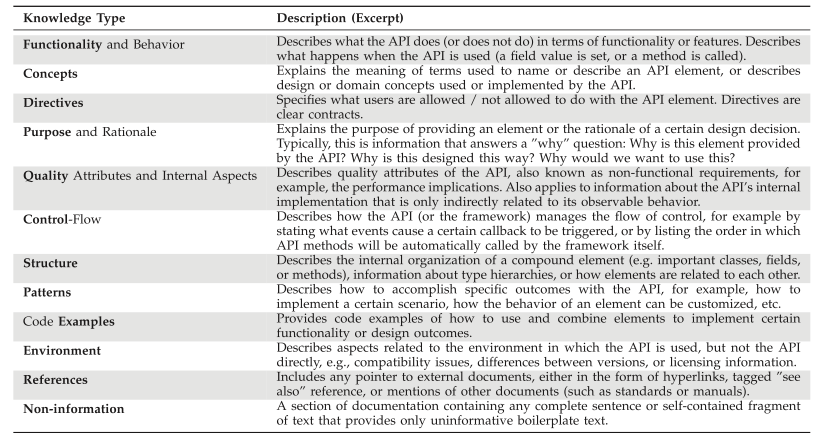
\includegraphics[width=1.1\textwidth]{pictures/knowledgetypes_original.png}
\caption[Wissenstypen in \cite{MaalejRobillard}]{Wissenstypen in \cite{MaalejRobillard}}
\label{fig:Wissenstypen_original}
\end{figure}
Die Vorgehensweise sah vor, dass die Gutachter f�r jeden Wissenstyp bestimmen, ob dieser in der vorgelegten Einheit vorkommt oder nicht. Hierzu konnten f�r jede Einheit die verschiedenen Wissenstypen mit Hilfe von "`CheckBoxes"' angekreuzt werden. 
Jede Einheit wurde von 2 Gutachtern unabh�ngig bewertet. Die Einheiten wurden in drei verschiedene Kategorieren aufgeteilt: 
\begin{enumerate}
\item Module [engl. modules] (entsprechen "`packages"' in Java und "`assemblies"' in .NET)
\item Typen [engl. types] (vor allem Klassen und Schnittstellen)
\item Mitglieder [engl. members] (Felder und Methoden)
\end{enumerate}
Die Einheiten der Kategorie "`Module"' wurden auf Grund der geringen Anzahl, der Unterschiedlichkeit (vor allem bzgl. der L�nge) in Java und .NET und des geringen Informatinosgehalts bei .NET dann aber nicht analysiert. Damit beschr�nkt sich die Original-Studie also auf Typen und Mitglieder. Die Stichprobe �ber die verbleibenden vier Kategorien (zwei je Programmiersprache) wurden mit 95\% Konfidenzintervall und 2,5\% Fehlerspanne gezogen, so dass insgesammt 5.575 Einheiten (431.136 W�rter) zuf�llig ausgew�hlt und auf 17 Gutachter verteilt wurden. \\
So sind insgesamt $5.574 * 2 = 11,148  $ Bewertungen vorgenommen worden. Diese wurden dann im Hinblick auf die �bereinstimmung unter den Gutachtern und bez�glich der Wissenstypen analysiert. Ebenso wurden Auswertungen �ber die F�lle getroffen, in denen sich zwei Gutachter uneinig waren. Zudem konnten so Aussagen dar�ber getroffen werden, welche Wissenstypen bei welcher Einheitskategorie wie h�ufig vorkommen und ob bestimmte Wissenstypen mit einander korrelieren, also  ob z.B. der Typ "'Structure"' h�ufig zusammen mit "`Functionality and Behaviour"' auftritt. Ebenso wurde analysiert, ob und wie ein Zusammenhang zwischen der Anzahl der gefundenen Wissenstypen und der L�nge der Einheiten besteht. \\
Besonders die vorgestellten Wissenstypen und das Kodier-Handbuch [Coding Guide] waren f�r diese Folgestudie sehr n�tzlich und wurden deswegen �bernommen und angepasst. 

\subsection{Kodier-Handbuch}
Das in der Original-Studie \cite{MaalejRobillard} verwendete Kodier-Handbuch findet auch in dieser Studie Verwendung, um von allen Gutachtern die selben bzw. sehr �hnliche Ergebnisse erwarten zu k�nnen. Es dient als Anleitung bei der Bewertung der Einheiten. W�hrend der Gro�teil des Handbuchs �bernommen wurde und unver�ndert bliebt, gab es jedoch ein paar wesentliche Anpassungen. 

\subsubsection{Markierungen}
\label{sec:Markierungen}
Der wichtigste Unterschied zu dem originalen Kodier-Handbuch \cite{codingguide_orig} ist, dass die Gutachtern nicht nur pro Einheit bewerten sollen, ob bestimmte Wissenstypen vorhanden sind, sondern Markierungen in einer Einheit vornehmen und pro Markierung einen Typ festlegen. Wie mit einem Textmarker soll jede Einheit vollst�ndig bearbeitet werden und abschlie�end jedes Zeichen (mit wenigen Ausnahmen) markiert sein. Dies f�hrt zu erg�nzenten Regeln �ber :
\begin{itemize}
\item Die Art Markierungen vorzunehmen
\item Der L�nge von Markierungen
\item Die Notwendigkeit von Doppelmarkierungen in einem Segment
\end{itemize}
Diese �nderungen wurden im ersten Absatz des Kodier-Handbuchs \cite{codingguide_new} wie folgt formuliert: 
\begin{shaded}
You will be presented with documentation blocks extracted from API reference documentation (Javadocs and the like). For each block, you will be also presented with the name of its corresponding package/namespace, class, method, or field. Your task is to read each block carefully and evaluate where the block contains knowledge of the different types described below. Apply the following rules when doing so:
\begin{itemize}
\item Consider the documentation initially one paragraph at a time. If the paragraph contains only information of one knowledge type, mark the whole paragraph with that type in one stretch.
Never mark more than one paragraph at once.
\item If multiple knowledge types mix within the paragraph, mark a contiguous stretch of one or more sentences with one type and the next stretch with another.
\item If necessary, treat subsentences connected with conjunctions such as "`and"', "`or"', "`but"', or with colon or semicolon like complete sentences.
\item A sentence (or such subsentence) as a whole is never marked with more than one type, but sometimes phrases within the sentence will require a separate marking with a different type. Double-marking the same text with two types is allowed (and required) in this case. To create such annotations uniformly, we work in two passes:
\begin{itemize}
\item Pass 1: Prefer longer segments of a complete sentence or several. Annotate subsentences only rarely.
If a sentence contains knowledge of more than one type (which happens quite often), look if one of them is clearly dominant for the overall role of the sentence in the documentation block. If so, annotate only that dominant type to the whole sentence and do not annotate any of the other types yet.
\item Pass 2: After pass 1, many relevant annotations will be missing. We now add those on top of the pass 1 annotations as double annotations. For the double annotations, we still prefer complete subsentences where possible (or other clearly delineated parts such as parentheses), but choose the shorter of two possibilities whenever we are unsure.
\end{itemize}
\item Rate the knowledge type as true only if there is clear evidence that knowledge of that type is present in the stretch.
If you have doubts, consult the type's definition below.
If the doubts do not disappear, do not annotate that type.
\item However, all text of the documentation must be marked with a type. (Only handwritten documentation, not the signature itself and not the placeholders [Something removed here] that indicate left-out nested documentation blocks).
\end{itemize}
Read (and re-read whenever needed) the following descriptions very carefully. They explain how to recognize each knowledge type.
\end{shaded}

\subsubsection{Kleinere �nderungen}
Zudem waren einige kleine �nderungen notwendig, die sich entweder aus dem Stil der Python-Dokumentation ergeben oder als sinnvoller bei der Bewertung von Einheiten ergeben haben. Folgende Semantische �nderungen gab es dabei: 

\begin{itemize}
\item Informationen �ber bestimmten Input einer Funktion oder Methode, welcher zu einer "`Exception"' f�hrt (und nur dann), soll als "`Directive"' und nicht als "`Functionality and Behavior"' markiert werden. 
\item Die simple Nennung von g�ltigen Parametertypen wird als nicht als "`Directive"' angesehen, sofern nicht  Schl�sselw�rter wie "`must"' oder "`have to"' etc. verwendet werden.
\item Der Ausdruck "`Changed in version x.y."' soll als "`Environment"' markiert werden. Der darauf anschlie�end Text kann ebenfalls "`Environment"' sein, muss es aber nicht. 
\item Platzhalter der Form "`[Something removed here]"' sollen nicht markiert und bewertet werden, da diese lediglich auf ausgelassene, verschachtelte Einheiten hinweisen (siehe Abschnitt "`Extrahierer"')
\item Der Wissenstyp "`Structure"' wird treffender in "`Structure and Relationship"' umbenannt. 
\end{itemize}



      
%\newpage
%\thispagestyle{empty}
%\mbox{}
%\newpage
\section{Konzeption}
In diesem Abschnitt werden grundlegende Faktoren und Vorgehenweisen erl�utert, die w�hrend der Bachelorarbeit wichtig geworden sind. 
Diese betreffen sowohl die Beschaffenheit der Dokumentionseinheiten als auch die Stichprobenziehung und der daraus resultierende Zeitaufwand f�r die Gutachter. 
\subsection{Dokumentationseinheiten}
Mit Dokumentationseinheiten werden die Teilabschnitte aus der Dokumentation bezeichnet, die ein Gutachter f�r die Bewertung zusammenh�ngend angezeigt bekommt. 
Diese Einheiten wurden anhand der HTML-Syntax in der Original-Dokumentation bestimmt. Es sind folgende Kategorien mit den dazugeh�rigen HTML?Syntaxen aufgetreten:
\begin{enumerate}
\item Methoden (engl. methods)
\begin{itemize}
\item <dl class=\grqq method\grqq>  Methodeninhalt </dl>
\item <dl class=\grqq classmethod\grqq>  Methodeninhalt </dl>
\item <dl class=\grqq staticmethod\grqq>  Methodeninhalt </dl>
\item <dl class=\grqq function\grqq>  Methodeninhalt </dl>

\end{itemize}
\item Felder (engl. fields)
\begin{itemize}
\item <dl class=\grqq attribute\grqq>  Feldinhalt </dl>
\item <dl class=\grqq data\grqq>  Feldinhalt </dl>
\end{itemize}
\item Module (engl. modules)
\begin{itemize}
\item <div class=\grqq section\grqq>  Modulinhalt </div>
\end{itemize}
\item Klassen (engl. classes)
\begin{itemize}
\item <dl class=\grqq class\grqq>  Klasseninhalt </dl>
\item <dl class=\grqq exception\grqq>  Klasseninhalt </dl>
\end{itemize}
\item Beschreibungen (engl. describe)
\begin{itemize}
\item <dl class=\grqq describe\grqq> Beschreibungstext </dl>
\end{itemize}
\end{enumerate}

Die Kategorien unterscheiden sich von denen aus der Originalstudie in der Form, dass Felder und Methoden unabh�ngig von einander gef�hrt werden und zus�tzlich noch die Beschreibungselemente hinzugekommen sind. Anders als in der Originalstudie wird die Kategorie Module in der sp�teren Analyse nicht ausgelassen. 
Die Einheiten unterscheiden sich nebst Inhalt auch stark in ihrer Textl�nge. W�hrend die Einheiten der Kategorien 1, 2,  4  und 5 tendenziell eine kleine Textl�nge haben, sind die Module (3. Kategorie) in der Regel l�nger:
\begin{figure}[H]
\centering
 \begin{bchart}[step=500,max=3400,scale=1.4]
  \bcbar[text=Methoden]{1225}
  \bcbar[text=Felder]{619}
  \bcbar[text=Module]{3385}
  \bcbar[text=Klassen]{1233}
  \bcbar[value=Beschreibungen 482]{482}  
 \end{bchart}
 \caption[Durchschnittliche Textl�ngen je Kategorie]{Durchschnittliche Textl�ngen je Kategorie}
\end{figure}

Sehr gro�e Unterschiede gibt es zudem in der H�ufigkeit verschiedener Typen. Die wenigsten Vorkommen gibt es von den Einheiten "`describe"', "`classmethod"' und "`staticmethod"'. Einheiten des Types "`Method"' treten dagegen am allerh�ufigsten auf. Trotz des geringen Auftretens der "`describe"'-Elemente haben wir uns daf�r entschlossen, diese als eigene Kategorie zu behandeln, da diese bei den bisher behandelten Programmiersprachen (Java und .NET) nicht existent waren.
\begin{figure}[H]
\centering
 \begin{bchart}[step=300,max=2500,scale=1.4]
  \bcbar[value=staticmethod 2]{2}
  \bcbar[value=describe 17]{17}
  \bcbar[value=classmethod 26]{26}
  \bcbar[value=exception 240]{240}
  \bcbar[text=class]{614}
  \bcbar[text=attribute]{748}
  \bcbar[text=data]{762}
  \bcbar[text=section]{1595}
  \bcbar[text=function]{1802}  
  \bcbar[text=method]{2565}
 \end{bchart}
  \caption[Gesamth�ufigkeiten der Einheiten]{Gesamth�ufigkeiten der Einheiten}
\end{figure}

Die Verteilung auf der Kategorie-Ebene zeigt ebenfalls einen deutlichen �berschuss an Methoden: n�mlich fast drei?mal so viele wie es Felder gibt.  Auf Grund der einelementigen Kategorien "`Module"' und "`Beschreibungen"' decken sich hier deren H�ufigkeiten exakt mit denen der "`section"' und "`describe"'-Einheiten, so dass auch hier die Beschreibungselemente den geringsten Anteil darstellen. 
\begin{figure}[H]
 \begin{bchart}[step=1000,max=4400,scale=1.4]
  \bcbar[text=Methoden]{4395}
  \bcbar[text=Felder]{1510}
  \bcbar[text=Module]{1595}
  \bcbar[text=Klassen]{854}
  \bcbar[value=Beschreibungen 17]{17}  
 \end{bchart}
  \caption[Gesamth�ufigkeiten der Kategorien]{Gesamth�ufigkeiten der Kategorien}
\end{figure}

Mit Hilfe dieser Informationen k�nnen die im n�chsten Abschnitt beschriebenen Stichprobengr��en berechnet werden. 
\subsection{Stichprobe}
Um f�r alle Kategorien ein aussagekr�ftiges Ergebnis der sp�teren Begutachtungen erzielen zu k�nnen, werden die Stichproben unter Vorgabe von Konfidenzintervall und Fehlerspanne separat von einander pro Kategorie gezogen.  
Die minimale Anzahl der pro Kategorien zu ziehenden Einheiten wird mit dieser Formel berechnet \cite{Stichprobenziehung}:
\begin{displaymath}
MIN = \frac{n_0}{1+\frac{n_0-1}{Gesamtmenge}} 
\end{displaymath}
wobei $n_0$ wie folgt berechnet wird: 
\begin{displaymath}
n_0 = \frac{Z^{2}*0.25}{e^{2}}
\end{displaymath}
Dabei ist Z die Angabe des Konfidenzintervalls als z-score und e die tolerierte Fehlerrate. 
Bei einem Konfidenzintervall von 95 Prozent ist Z=1.96 \cite{Stichprobenziehung}. 
Mit einer Fehlerrate von 5 Prozent ergibt sich f�r $n_0 = 384,16$ und dadurch dann die folgenden minimale Stichprobengr��en f�r die jeweiligen Kategorien: \newline
\begin{figure}[H]
\centering
\begin{tabular}{|c||c|c|}\hline
   Kategorie & Gesamtmenge & Stichprobengr��e\\ \hline \hline
   Methoden & 4395 & 651 \\ \hline
   Felder & 1510 & 306\\ \hline
   Module & 1595 & 310 \\ \hline
   Klassen & 854 & 265 \\ \hline
   Beschreibungen & 17 & 16 \\ \hline \hline
   \textbf{Summe} & 8371 & 1548 \\ \hline
 \end{tabular}
\caption[Stichprobengr��en]{Stichprobengr��en}
\end{figure}
\subsection{Goldstichprobe}
Zudem wurde so eine weitere Stichprobe, die Goldstichprobe gezogen. Diese hat folgenden Zweck: 
\begin{itemize}
\item Absicherung der Messung bez�glich Korrektheit der Gutachterergebnisse und
\item Bestimmung eines Wertes f�r hohe Typisierungsqualit�t 
\end{itemize}
Diese Stichprobe wurde dann von vier unabh�ngigen Gutachtern der Freien Universit�t Berlin (Institut f�r Informatik) jeweils vollst�ndig typisiert. Diese Gutachter waren:
\begin{itemize}
\item Prof. Dr. Lutz Prechelt, AG Software Engineering
\item Holger Schmeisky, AG Software Engineering 
\item Franz Zieris, AG Software Engineering
\item Sven Wildermann, Verfasser dieser Bachelorarbeit
\end{itemize}
Wobei Holger Schmeisky und Franz Zieris zusammen eine Stichprobe bearbeitet haben. 
\newline
Die Gr��e dieser Stichprobe wurde auf 2 Prozent der Gesamtmenge aller Einheiten festgelegt, damit bei Beibehaltung einer repr�sentativen Gr��e der Aufwand im Rahmen blieb. F�r die einzelnen Kategorien ergaben sich somit folgende Mengen: 
\begin{figure}[H]
\centering
\begin{tabular}{|c||c|c|}\hline
   Kategorie & Gesamtmenge & Stichprobengr��e\\ \hline \hline
   Methoden & 4395 & 88 \\ \hline
   Felder & 1510 & 30 \\ \hline
   Module & 1595 & 32 \\ \hline
   Klassen & 854 & 17 \\ \hline
   Beschreibungen & 17 & 1 \\ \hline \hline
   \textbf{Summe} & 8371 & 168 \\ \hline
 \end{tabular}
\caption[Goldstichprobengr��en]{Goldstichprobengr��en}
\end{figure}
Dabei wurde der Wert f�r die Kategorie "`Beschreibungen"' um eins erh�ht, da diese Elemente sonst �berhaupt nicht in der Goldstichprobe vorgekommen w�ren. 
\subsection{Zeitaufwand}
Da die Gutachter der Hauptstichprobe im Rahmen des Kurses "`Forschungspraktikum"' an der Freien Universit�t Berlin f�r f�nf ECTS \footnote{European Credit Transfer System} die Einheiten bewerten haben, sollte der Aufwand so verteilt werden, dass die ben�tigten Punkte erreicht werden, aber gleichzeitig der Zeitaufwand nicht �berschritten wird (ein ECTS entspricht etwa 25 bis 30 Arbeitsstunden). Hierf�r muss der Aufwand des Markierens pro Einheit gesch�tzt werden, so dass die Einheiten pro Gutachter festgelegt werden k�nnen. Diese �berlegungen sind auch schon in der Stichprobenziehung mit eingeflossen und haben dazu gef�hrt, dass die Fehlerrate auf 5 Prozent gesetzt wurde. Da vor dem Start noch eine intensive Einarbeitung inklusive Hausarbeiten durchgef�hrt wurde, sind f�r die eigentliche Bewertung der Einheiten noch drei ECTS pro Student veranschlagt worden. Dadurch, dass jede Einheit von zwei Gutachtern bewertet werden sollte, mussten vorher die Stichprobengr��en mit zwei multipliziert werden, um die Gesamtanzahl der Bewertungen zu erhalten. Diese wurde dann auf die sieben Studenten verteilt (in der Tabelle wurde gerundet) und mit einem grob gesch�tzten, durchschnittlichen Zeitaufwand pro Einheit multipliziert: 
\begin{figure}[H]
\centering
\begin{tabular}{|c||c|c|c|c|}\hline
    & Anzahl der & Einheiten & Zeitaufwand & Zeitaufwand\\
   Kategorie & Bewertungen & pro Student & pro Einheit & gesamt\\ \hline \hline
   Methoden & 1302 & 186  & 5 min & 930 min \\ \hline
   Felder &  12 & 87 & 5 min & 435 min\\ \hline
   Module & 620 & 89 & 15 min & 1335 min\\ \hline
   Klassen &  530  & 76 & 10 min & 760 min\\ \hline
   Beschreibungen &  32 & 5 & 3 min & 15 min\\ \hline \hline
   \textbf{Summe} &  3096  & 443 & $\oslash 7.6$ min&  57,92 h\\ \hline
 \end{tabular}
\caption[Einheiten pro Student inkl. Zeitaufwand]{Einheiten pro Student}
\end{figure}
Zus�tzlich waren die Gutachter dazu angehalten, regelm��ig das KodierHandbuch zu lesen, um das �bergreifende Verst�ndnis nicht zu verlieren, sowie gelegentlich mit dem BugTracker\footnote{Ein System zur Erfassung von Defekten und Verbesserungsvorschl�gen} umzugehen. Hierf�r wurden zus�tzlich insgesamt noch etwa zehn bis zwanzig Arbeitsstunden invenstiert, wobei der tats�chliche Aufwand je Gutachter stark abweichen kann. \\
\newline
Analog kann auch der Zeitaufwand f�r die Bearbeitung der Goldstichprobe berechnet werden: 
\begin{figure}[H]
\centering
\begin{tabular}{|c||c|c|c|c|}\hline
                    & Anzahl der & Zeitaufwand & Zeitaufwand\\
   Kategorie & Einheiten &  pro Einheit & gesamt\\ \hline \hline
   Methoden & 88 &  5 min & 440 min \\ \hline
   Felder &  30 &  5 min & 150 min\\ \hline
   Module & 32 &  15 min & 480 min\\ \hline
   Klassen &  17  &  10 min & 170 min\\ \hline
   Beschreibungen &  1 & 3 min & 3 min\\ \hline \hline
   \textbf{Summe} &  168  & $\oslash 7.6$ min&  20,72 h \\ \hline
 \end{tabular}
\caption[Zeitaufwand f�r die Goldstichprobe]{Zeitaufwand f�r die Goldstichprobe}
\end{figure}
Da die Goldstichprobe drei mal bearbeitet wurde, ergibt sich so ein Gesamtaufwand f�r die Bearbeitung dieser von 62,16 Stunden.
Somit stellt sich die Frage, wie diese Einheiten aus der Original?Dokumentation verf�gbar gemacht werden.
\subsection{CADo-Tool vs. Eigenentwicklung}
Im Rahmen der Forschung von Maalej und Robillard \cite{MaalejRobillard} wurde ein Tool mit dem Namen CADo\footnote{Content Analysis for Software Documentation} geschaffen, welches folgende Werkzeuge und folgendee F�higkeiten mit sich bringt (�bersetzter Auszug) \cite{cado_tool} :
\begin{itemize}
\item API-Dokumentionen aus Online-Quellen extrahieren
\item Ziehen von zuf�lligen, stratifizierten Stichproben
\item Erstellung eines Codierungsschemas
\item Zuweisen von Einheiten zu Gutachtern
\item Berechnung der �bereinstimmung von Gutachtern
\end{itemize}
Aus der Perspektive des Gutachters birgt dieses Tool zus�tzlich noch folgende F�higkeiten \cite{cado_tool}:
\begin{itemize}
\item Online und offline login
\item Laden der zugewiesenen Einheiten
\item Einheiten typisieren (Codierungen hinzuf�gen)
\item Kodierhandbuch anzeigen 
\item Darstellung der Dokumentation
\item Kodiersitzungen zwischenspeichern und laden
\item Statistiken ansehen
\end{itemize}

Auf Grund der Vielzahl der f�r uns n�tzlichen F�higkeiten, stellte sich die Frage, ob dieses Werkzeug f�r diese Bachelorarbeit ebenfalls genutzt werden kann. 
Also habe ich dieses Werkzeug heruntergeladen und ausprobiert. Schon beim Herunterladen gab es Schwierigkeiten, da der auf der Website ver�ffentlichte Link ung�ltig war. Nach R�ckfragen bei den Autoren wurde dieser Misstand dann innerhalb weniger Tage von diesen behoben. \\
Der Test des Werkzeugs erwies sich dann ebenfalls als schwierig, da es noch in der alpha-Version\footnote{fr�hes Entwicklungsstadium ohne Garantie auf fehlerfreies funktionieren} und ohne Benutzerhandbuch vorlag. Zudem gab es bei m�glichen Fragen keinen einheitlichen Ansprechspartner und keine garantierte Antwortzeit der Entwickler, was ebenfalls zu einem h�herem Risikio in der Benutzung gef�hrt h�tte. \\
Somit haben wir es als sinnvoller angesehen, die f�r diese Bachelorabeit ben�tigten Werkzeuge selbst zu entwickeln. Dies hatte noch weitere Vorteile: 
\begin{itemize}
\item Grundverst�ndnis des vorliegenden Programmcodes
\item �nderungen des Grundkonzepts eher m�glich
\item schnellere Weiterentwicklung bei Bedarf
\item weniger Kommunikationsaufwand 
\end{itemize}
Wir haben uns entschlossen, diese Werkzeuge dann mittels Python zu entwicklen, um zus�tzlich noch Synergieeffekte bez�glich des Erlernens und Verstehens der Programmiersprache Python auszunutzen. 
\\ 
Da der Zugriff verteilt von den Rechnern der Gutachter erfolgen sollte, war die Entwicklung einer Website zu diesem Zweck sinnvoll, so dass Restriktionen bez�glich der Betriebssystemwahl ausger�umt werden konnten. \\
Diese Entscheidung f�hrte dazu, dass wir die Typisierungen �berhaupt anhand von Markierungen durchf�hren konnten (siehe Erl�uterung in Kapitel \ref{sec:Markierungen}), da wir so nicht mehr an den Gegebenheiten des CADo-Tools gebunden waren.

\section{Entwicklung und Durchf�hrung}
In diesem Kapitel wird zuerst erl�utert, wie das Extrahieren der Dokumentationseinheiten aus der Original?Pythondokumentation gemeistert wurde. Anschlie�end wird die Konzipierung und Umsetzung des Werkzeugs f�r die Markierung der Dokumentationseinheiten besprochen.
\subsection{Extrahierer}
Um die Dokumentationseinheiten aus der HTML-Dokumentation von Python zu erhalten, war es n�tig, einen Extrahierer als Skript zu schreiben. Dieser wurde in Python3 mit Hilfe von BeautifulSoup4 angefertigt. BeautifulSoup wurde genutzt, da es im Gegensatz zu regul�ren Ausdr�cken eine verst�ndlichere Syntax bietet, was zu einer leichteren und wartbareren Entwicklung f�hrt. \\
Entsprechend der Definitionen von Dokumentationseinheiten sollten also die HTML-Schnipsel getrennt von einander in eine Datenbank importiert werden. Diese Einheiten sind allerdings h�ufig geschachtelt, so dass eine Methodendeklaration in der Regel innerhalb einer Klassenbeschreibung vorkommt, welche wiederum innerhalb einer Sektion anzutreffen ist. Um Dopplungen bei der Typisierung zu vermeiden, wurden deswegen Platzhalter der Form "`[something removed here]"' an solchen Stellen eingebaut. Platzhalter haben einen wichtigen Vorteil gegen�ber dem einfachen Weggelassen dieser Elemente. So sieht auch der Gutachter, dass hier etwas von der Original-Dokumentation abweicht und kann sich somit die entstandenen L�cken erkl�ren. Dieser Fall tritt besonders h�ufig bei Sektionen auf, da diese in der Regel alle weiteren Elemente beinhalten. Aneinanderreihungen von Platzhaltern wurden wieder zu einem Platzhalter zusammengefasst.  \\
Eine m�gliche Struktur der Verschachtelung von Dokumentationseinheiten sieht ohne Beschr�nkung der Allgemeinheit so aus:  
\begin{figure}[H]
\centering
\begin{tikzpicture}[
  level 1/.style={sibling distance=40mm},
  edge from parent/.style={->,draw},
  >=latex]

% root of the the initial tree, level 1
\node[root] {section}
% The first level, as children of the initial tree
  child {node[level 2] (c1) {section}}
  child {node[level 2] (c2) {class}}
  child {node[level 2] (c3) {section}};

% The second level, relatively positioned nodes
\begin{scope}[every node/.style={level 3}]
\node [below of = c1, xshift=15pt] (c11) {function};
\node [below of = c11] (c12) {function};
\node [below of = c12] (c13) {function};
\node [below of = c13] (c14) {exception};

\node [below of = c2, xshift=15pt] (c21) {method};
\node [below of = c21] (c22) {attribute};
\node [below of = c22] (c23) {data};
\node [below of = c23] (c24) {data};

\node [below of = c3, xshift=15pt] (c31) {section};
\node [below of = c31] (c32) {section};
\end{scope}

% lines from each level 1 node to every one of its "children"
\foreach \value in {1,...,4}
  \draw[->] (c1.195) |- (c1\value.west);

\foreach \value in {1,...,4}
  \draw[->] (c2.195) |- (c2\value.west);

\foreach \value in {1,...,2}
  \draw[->] (c3.195) |- (c3\value.west);
\end{tikzpicture}
\caption{Beispielhafte Struktur der HTML-Elemente}
\label{fig:HTML-Elemente}
\end{figure}
\subsubsection{BeautifulSoup4}

F�r das Parsen der HTML-Einheiten wurde BeautifulSoup4 verwendet, da es ein hierf�r geschaffenes, m�chtiges Werkzeug darstellt und gleichzeitig auf Python basiert. Somit konnte ich Synergieeffekte nutzen und mich w�hrend des Schreibens am Skript weiter in Python einarbeiten. Zudem bietet der Einsatz von BeautifulSoup viele Vorteile gegen�ber dem Parsen mittels regul�ren Ausdr�cken. In erster Linie ist der Code lesbarer und verst�ndlicher, sowohl f�r den Entwickler selbst als auch f�r Dritte. Au�erdem gibt es eine ausf�hrliche Dokumentation inklusive zahlreicher Beispiele und auch die Community hinter BeautifulSoup ist gro� genug, um auf Internetportalen wie \href{http://www.stackoverflow.com}{Stackoverflow}\footnote{www.stackoverflow.com} Unterst�tzung erhalten zu k�nnen.  Die Implementierung selbst wird im nachfolgenden Kapitel erkl�rt. 

\subsubsection{Implementierung}

Bevor die n�tigen Schritte mit BeautifulSoup4 durchgef�hrt werden konnten, war es n�tig, die vollst�ndige Dokumentation herunterzuladen und die notwendigen Dateien ausfindig zu machen. Unter dem Link \url{https://docs.python.org/3.4/archives/python-3.4.1-docs-html.zip} ist die gesamte Dokumentation in einem HTML?Format verf�gbar. Interessant sind jedoch lediglich die Dateien in dem Unterordner "`library"' innerhalb dieser ZIP?Datei,  da Tutorials, Inhaltsverzeichnisse, FAQ und zus�tzliche Informationen analog der Studie von Maalej und Robillard \cite{MaalejRobillard} ausgeschlossen wurden. \newline

Der Extrahierer durchsucht anfangs alle Dateien in dem Unterordner "`library"' und f�gt den vollst�ndigen Pfad in eine Liste:
\lstinputlisting[language=Python, firstline=91, lastline=92]{code/extractor.py}

Aus jeder Datei wird dann ein BeautifulSoup-Objekt gemacht, welches die verschachtelte, innere HTML-Datenstruktur repr�sentiert:
\lstinputlisting[language=Python, firstline=94, lastline=95]{code/extractor.py}
Dieser Schritt ist n�tig, um im Anschluss mittels BeautifulSoup-API die einzelnen Dokumentationseinheiten extrahieren zu k�nnen. Hierf�r wird der Befehl find-all genutzt. Um eine einfache und fehlerfreie Bedienung zu erm�glichen, wurde eine Funktion geschrieben, die das DOM\footnote{Document Object Model}-Element samt Attribute entgegen nimmt:
\lstinputlisting[language=Python, firstline=84, lastline=86]{code/extractor.py}
Der Aufruf zum Parsen alle Elemente der Form 
\begin{lstlisting} 
<dl class="method"> 
Inhalt des Elements
</dl>
\end{lstlisting} 
und abspeichern dieser in einer Liste funktioniert dann wie folgt:
\lstinputlisting[language=Python, firstline=99, lastline=99]{code/extractor.py}
Dieser Schritt wurde analog f�r alle zehn verschiedenen Elementsytpen ausgef�hrt. 
Um sp�ter Aussagen �ber die Lage der Texte innerhalb einer Einheit zu erhalten, wurden zudem die Startoffsets der Elemente berechnet und sp�ter zusammen mit dem Endoffsets in der Datenbank abgelegt, wobei sich das Endoffset jeweils sehr leicht errechnen l�sst: 
$ Ende = Start + Laenge$.\\
F�r die Bestimmung der Startoffsets wurden die einzelnen Elemente in ihrer Datei mittels "`find"' aus BeautifulSoup gesucht und die R�ckgabe, also der Index an der Stelle des Auftretens, gespeichert. Auch hierf�r gibt es eine eigene Funktion, um den Aufruf lesbarer zu gestalten: \\ \\
\begin{minipage}{\textwidth}
 \lstinputlisting[language=Python, firstline=28, lastline=36]{code/extractor.py}
\end{minipage}
\newline
Au�erdem wurde dann f�r jedes Element das Vaterelement gesucht. Zum einen, um die Elemente sp�ter leichter wieder in die richtige Reihenfolge bringen zu k�nnen und zum anderen, um den Gutachtern die M�glichkeit zu geben, sich den engeren Kontext, in dem die zu bewertende Einheit steht, genauer anzusehen: 
 \lstinputlisting[language=Python, firstline=63, lastline=65]{code/extractor.py}
Wegen der bereits erw�hnten, verschachelten HTML-Struktur der Elemente musste ein Weg gefunden werden, um zu verhindern, dass ein inneres Element zweimal von den Gutachtern typisiert wird. Also wurden alle Vorkommen von inneren Elementen in den �u�eren Elemente durch folgende Platzhalter ersetzt: 
  \lstinputlisting[language=Python, firstline=138, lastline=138]{code/extractor.py}
Da so in vielen F�llen, z.B. bei der Aufz�hlung von Methoden und Attributen,  seitenweise Platzhalter entstanden w�ren, wurden im Anschluss direkt aufeinander folgende Platzhalter wieder zu einem Platzhalter zusammengefasst:
  \lstinputlisting[language=Python, firstline=39, lastline=44]{code/extractor.py}
Die final zur Verf�gung stehenden Informationen wurden dann in einer Datenbank abgespeichert.

\subsection{Typisierungswebsite}
% Die Typisierungwebsite stellt den Zugang f�r alle Gutachtern zu den Dokumentationseinheiten dar.
\subsubsection{Anforderungen}
Damit die Einheiten von den Studenten typisiert werden konnten, musste ein Werkzeug geschaffen werden, welches folgende Eigenschaften aufweist. Die mit einem Stern markierten Eigenschaften sind optional:
\begin{itemize}
\item Ein- und Auslogfunktion
\item Betriebssystemunabh�ngige Online-Erreichbarkeit
\item Anzeige der dem Student zugewiesenen Einheiten
\item Markierung von Segementen und Zuweisung zu Informationstypen
\item Anzeige der gesetzten Markierungen * 
\item Anzeige der Anzahl noch verbleibender und schon gespeicherter Einheiten *
\item Anzeige der eigenen �bereinstimmung mit anderen Studenten * 
\end{itemize}

\subsubsection{Umsetzung}
F�r die Umsetzung der genannten Anforderungen wurde das Webframework "`Django"' verwendet ? da es auf "`Python"' basiert und es eine gro�e Community gibt, die im Zweifel bei Herausforderungen unterst�tzten k�nnen. F�r die Beantwortung der anf�nglichen Fragen haben wir das in Berlin stattfindende Meetup der Django User Group\footnote{http://www.meetup.com/django-user-group-berlin/} besucht. Dar�ber hinaus gibt es eine Vielzahl von M�glichkeiten, mit anderen Django-Entwicklern zu kommunizieren, wie �ber die Mailingliste\footnote{{https://groups.google.com/forum/\#!forum/django-de}} oder den IRC-Chat (deutsch/weltweit).
\paragraph{Navigationsleiste} $\;$ \\
Die Navigationsleiste soll dem jeweiligen Benutzer alle Funktionen und Seiten anzeigen, die er im Rahmen des Werkzeugs benutzen kann.
Links, die auf ein Ziel innerhalb des Werkezeugs f�hren, sind blau. Externe Links sind grau gestaltet. 
Administrator-Funktionalit�ten haben eine rote Linkfarbe und werden nur eingeloggten Administratoren angezeigt. Wenn ein Benutzer ohne Administrationsrechte dennoch auf einen Link ger�t, f�r dessen Inhalt er keine Berechtigung besitzt, wird eine entsprechende Benachrichtigung angezeigt.

\paragraph{Login} $\;$ \\
Der Login soll allen Gutachtern erm�glichen, sich mit einem individuellen Account anzumelden, um gesch�tzten Zugriff auf die Dokumentationseinheiten und die pers�nliche Statistik zu erhalten. Weiterhin sollen Administratoren sich �ber diese Maske anmelden k�nnen, um Zugriff auf Administratorfunktionalit�ten zu erhalten. \newline
Der Login-Bereich wurde mit Hilfe des bereits in Django vorhandenen Authentifizierungsmoduls gefertigt. Angepasst wurde das Design an das der restlichen Website. Da eine Funktion f�r das Zur�cksetzten des Passwortes nicht ben�tigt wurde, wurde diese auch nicht implementiert. 
\begin{figure}[H] 
\centering
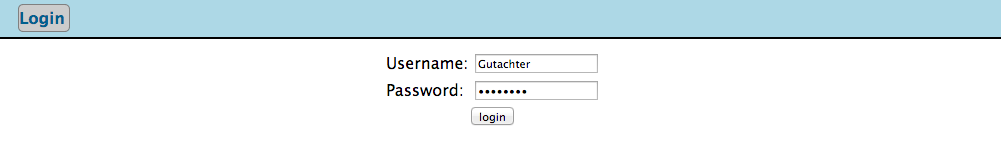
\includegraphics[width=1.0\textwidth]{pictures/login.png}
\caption[Login-Bereich]{Login-Bereich}
\label{fig:Login}
\end{figure}
$\;$ \\
\paragraph{Einheit typisieren} $\;$ \\
Nach dem Login wird der Gutachter direkt zu der n�chsten zu typisierenden Einheit weitergeleitet. 
Auf dieser werden neben der Navigation noch die Identifikationsnummer der Dokumentationseinheit, der Text der Einheit und Steuerungselemente angezeigt. Die Steuerungselemente sind im Einzelnen: 
\begin{enumerate}
\item Save ? speichert die aktuelle Markierung
\item Delete All ? l�scht alle gesetzten Markierungen des Gutachter bei dieser Einheit
\item Show Parent ? zeigt das direkte Vaterelement der Dokumentationseinheit an (siehe Abbildung \ref{fig:HTML-Elemente})
\item Show File ? zeigt die gesamte HTML-Datei, aus welcher diese Dokumentationseinheit stammt, im Original an
\end{enumerate}
Sobald der Text von dieser Einheit mit dem Mauscursor markiert wurde, erscheint ein Fenster f�r die Auswahl eines Wissenstypes. 
Die Position der Markierung wird dann zusammen mit dem Wissenstyp mit Hilfe von Javascript zwischengespeichert und dann beim Klicken auf "`save"' �ber Ajax als POST-request an den Controller\footnote{Entsprechend des "`Model View Controller"'-Musters} (in Django ist es die views.py) gesendet. Nach dem Speichern wird dann die n�chste Einheit angezeigt.  $\;$ \\
\begin{figure}[H] 
\centering
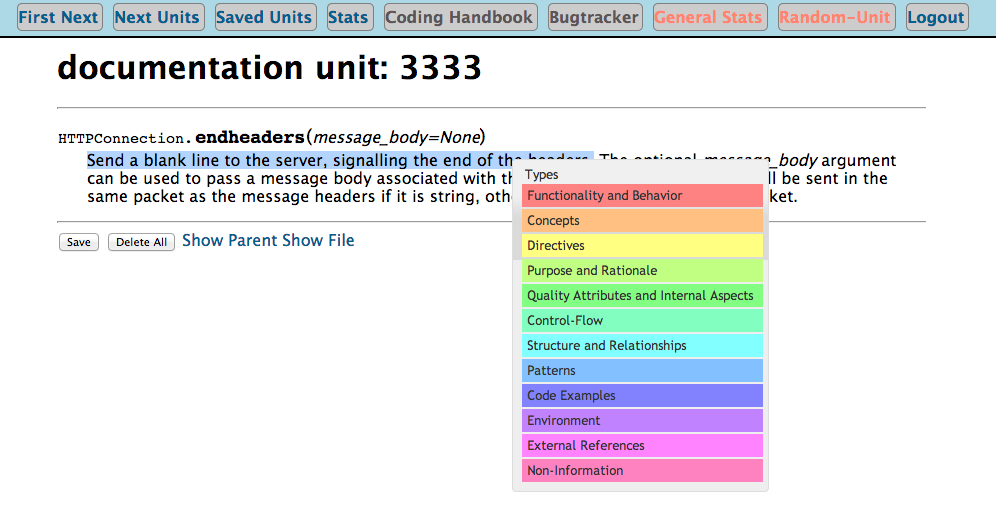
\includegraphics[width=1.0\textwidth]{pictures/marking.png}
\caption[Einheit typisieren]{Einheit typisieren}
\end{figure}
$\;$ \\
Die gesetzten Markierungen werden mit JavaScript farblich dargestellt. Bei Doppelmarkierungen wird die Farbe angezeigt, die zuletzt f�r die Auswahl gew�hlt wurde. Au�erdem erscheint unterhalb der Einheit eine Auflistung aller Markierungen. Sobald ein Element aus dieser Auflistung mit Mouse-Over\footnote{Bewegung des Maus-Cursor auf ein Element ohne es anzuklicken} ber�hrt wird, wird der damit verbundene, markierte Text rot und gestrichelt umrandet. Ein Klick auf dieses Element bewirkt das L�schen der angezeiten Markierung. 
\begin{figure}[H] 
\centering
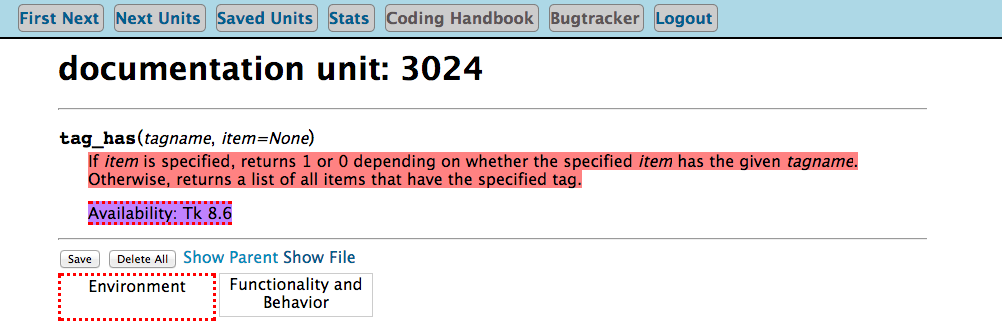
\includegraphics[width=1.0\textwidth]{pictures/single-delete.png}
\caption[Einheit typisieren (2)]{Einheit typisieren (2)}
\end{figure}
\paragraph{Noch nicht typisierte Einheiten} $\;$ \\
F�r den Fall, dass der Gutachter die zur Zeit n�chste Einheit noch nicht bewerten will, weil ihm diese f�r den Augenblick zu lang erscheint oder ihm gerade zu schwierig ist, kann er sich alle Einheiten auflisten, die noch typisiert werden m�ssen und davon eine ausw�hlen, die er als n�chstes bearbeiten m�chte. Dabei wird dem Gutachter die Identifikationsnummer, die Datei aus welcher die Einheit kommt und die Kategorie angezeigt. Der Klick auf eine Zeile f�hrt dann zu der Maske, in welcher die Einheit typisiert werden kann.
\begin{figure}[H] 
\centering
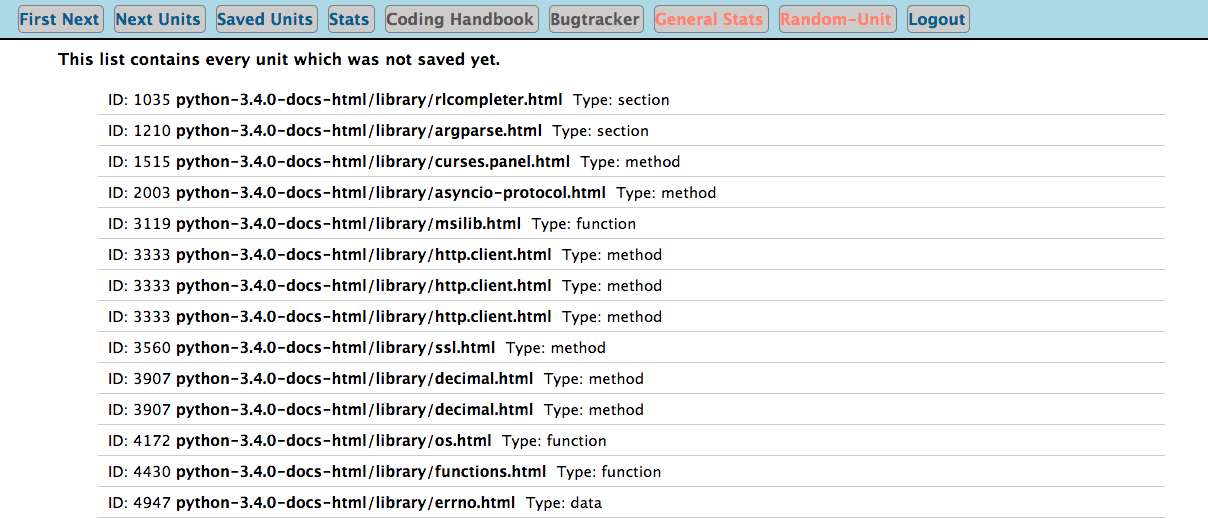
\includegraphics[width=1.0\textwidth]{pictures/list_of_next.png}
\caption[Noch nicht typisierte Einheiten]{Noch nicht typisierte Einheiten}
\end{figure}

\paragraph{Typisierte Einheiten} $\;$ \\
Zudem kann sich der Gutachter alle Einheiten auflisten lassen, die er bereits typisiert hat. Dabei werden alle Einheiten gelb hervorgehoben, die zu mehr als 25 Prozent und mehr als 100 Zeichen nicht markiert sind. Dies wurde so eingef�hrt, damit sehr kurze Einheiten, bei denen die nicht zu typisierende �berschrift fast genauso lang ist wie der eigentliche Text, nicht f�lschlich hervorgehoben werden. Bei den Textl�ngen wurden au�erdem die eingef�hrten Platzhalter herausgerechnet, da auch diese nicht markiert werden sollten.
So hat der Gutachter eine schnelle �bersicht �ber Einheiten, die er (in der Regel versehentlich) unvollst�ndig abgespeichert hat. 
Weiterhin wird f�r jede Einheit der Zeitstempel der vorhergegangenen Speicherung ausgegeben und bei Hervorhebung noch die Angabe in Prozent, wie viel des Textes nicht markiert ist. 
\begin{figure}[H] 
\centering
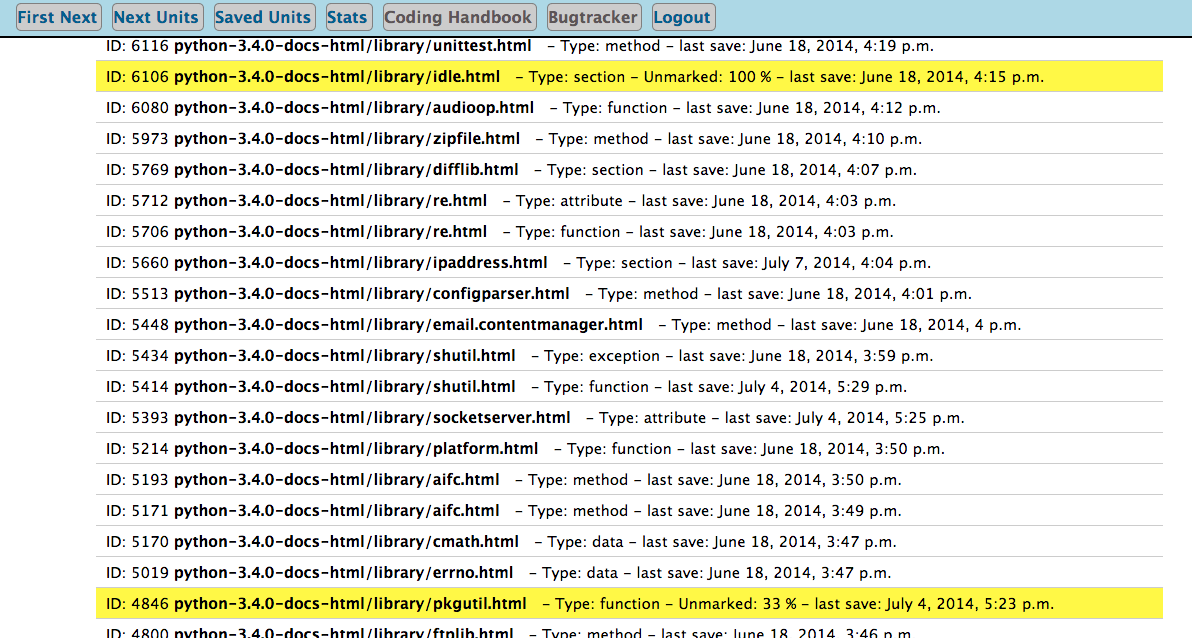
\includegraphics[width=1.0\textwidth]{pictures/einheiten-gespeichert.png}
\caption[Abgespeicherte Einheiten]{Abgespeicherte Einheiten}
\end{figure}
\paragraph{Pers�nliche Statistik} $\;$ \\
In der Statistik  (kurz: Stats) werdem dem angemeldeten Benutzer folgende Werte angezeigt: 
\begin{enumerate}
\item Anzahl insgesamt abgespeicherter Einheiten
\item Anzahl noch zu typisierender Einheiten (noch nicht abgespeichert)
\item Anzahl insgesamt zugewiesener Einheiten
\item Prozentuale �bereinstimmung der Markierungen mit den anderen Gutachtern (nur f�r die Gutachter der Hauptstichprobe)
\item Angabe der Anzahl der Einheiten, auf die sich die Berechnung der �bereinstimmung st�tzt
\end{enumerate}
Die 5. Angabe ist deswegen wichtig, da die Berechnung bei den schnellen Gutachtern sich auf weniger Einheiten st�tzt als schon markiert wurden. 
Das ist der Tatsache geschuldet, dass die Berechnung der �bereinstimmung pro Einheit erst erfolgen kann, wenn zwei Gutachter diese abgespeichert haben.\\
Diese Angaben werden einmal im Gesamten gemacht und dann anhand der letzten Speicherungsdaten f�r die letzten vierzehn, acht, vier und zwei Tage. Das hat den Vorteil, dass jeder Student schnell seinen eigenen Fortschritt f�r eine kurze Vergangenheit beobachten und dann auch ggf. erkennen kann, ob die �bereinstimmung mit anderen Gutachtern eher zu- oder abnimmt. \\ 
\begin{figure}[H] 
\centering
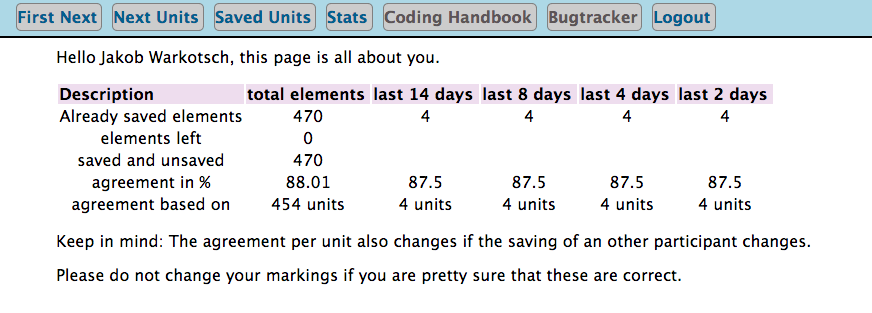
\includegraphics[width=1.0\textwidth]{pictures/personal_stats.png}
\caption[Pers�nliche Statistik]{Pers�nliche Statistik}
\end{figure}

\paragraph{Kodierhandbuch} $\;$ \\
Aus der Websitenavigation heraus kann direkt das Kodierhandbuch in einem neuen Tab ge�ffnet werden. Der Link verweist direkt auf die Website, die dieses enth�lt. 
Dieser direkte Link soll dazu f�hren, dass nochmaliges nachlesen m�glichst einfach gemacht wird und die Gutachter nicht erst noch nach dem Link suchen m�ssen. 
Der Link ist in der Navigation grau markiert, um zu verdeutlichen, dass es sich dabei um eine externe URL handelt.
\paragraph{Bugtracker} $\;$ \\
Ebenso kann der Bugtracker (gehosted bei bitbucket.org) schnell aus der Navigation heraus erreicht werden. Die Gutachter wurden angehalten, Schwierigkeiten in der Bedienung oder auftretende Fehler direkt dort zu melden, so dass alle Aufgaben bez�glich Verbesserung der Website zentral verwaltet werden k�nnen. Gegen�ber der �blichen E-Mail-Kommunikation hat dies den Vorteil, dass Gutachter erkennen k�nnen, wenn ein Fehler bereits gemeldet wurde, so dass Dubletten vermieden werden k�nnen. Au�erdem k�nnen Gutachter noch zus�tzliche Informationen zu den einzelnen Aufgaben liefern und f�r die Erledigung einer Aufgabe stimmen. \\
Weiterhin kann der interessierte Gutachter sich hier�ber den gesamten Quelltext der Website ansehen und so Ursache und L�sung der einzelnen Thematiken nachvollziehen, denn �nderungskommentare sind so in der Regel mit der l�senden �nderung im Quelltext verkn�pft. 
\begin{figure}[H] 
\centering
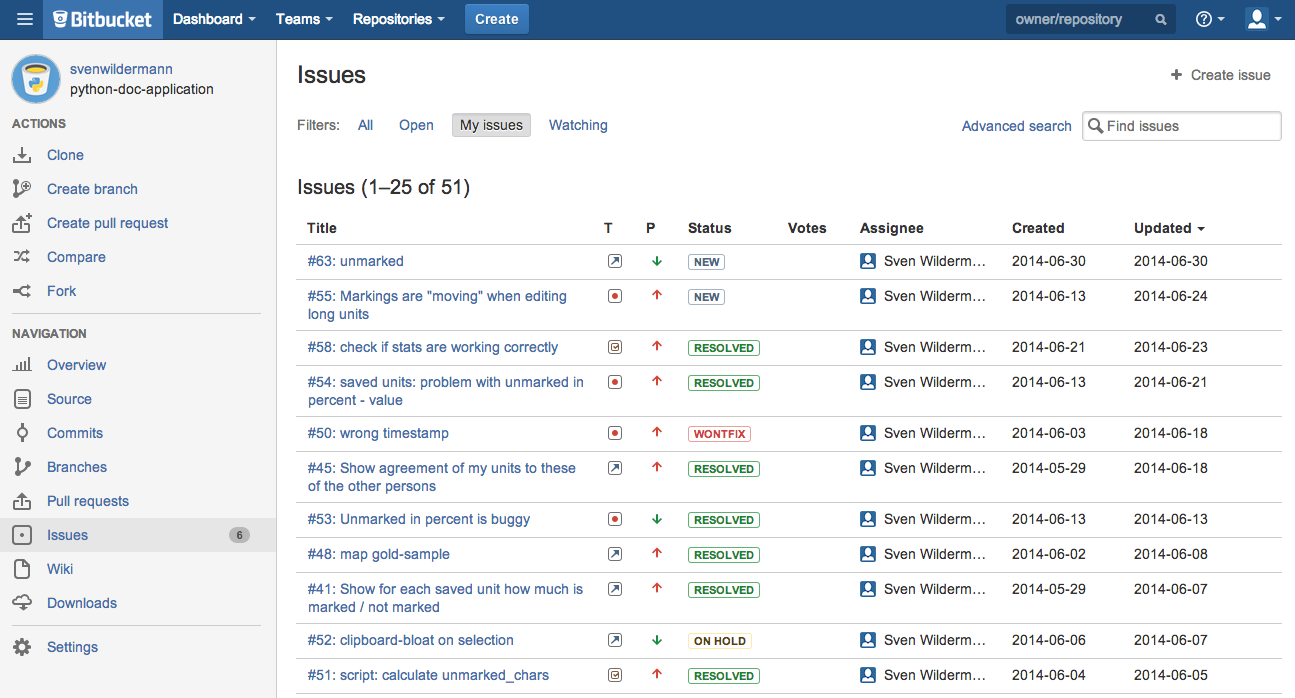
\includegraphics[width=1.0\textwidth]{pictures/bitbucket.png}
\caption[Bugtracker]{Bugtracker}
\end{figure}

\paragraph{Allgemeine Statistik} $\;$ \\
Die allgemeine Statistik ist eine reine Administratorfunktionalit�t und zeigt im wesentlichen die pers�nliche Statistik f�r alle Gutachter �bersichtlich an. Die �bereinstimmung unter den Gutachtern der Goldstichprobe wurde nicht berechnet und deswegen auch nicht angezeigt. Au�erdem weist diese Statistik noch die insgesamt zugewiesenen, gespeicherten (auch ohne Markierungen), markierten und nicht gespeicherten Einheiten an. Dabei werden Einheiten von Test- und Administratoraccounts mitberechnet. Da die einzelnen Gutachter hier mit Vornamen aufgelistet werden, wird auf die Einbindung eines Screenshots aus Datenschutzgr�nden verzichtet. 
\paragraph{Zuf�llige Einheit} $\;$ \\
Der "`Random Unit"'-Button ist ebenfalls eine reine Administratorfunktionalit�t und dient lediglich dem Testen. Grund f�r die Einf�hrung dieses Buttons war, dass bei Neuentwicklungen immer wieder anhand bisher unmarkierter Einheiten getestet werden und f�r die Zuweisung jedes Mal die Terminalumgebung genutzt werden musste. \\
Im Wesentlichen ist hinter dieser Funktion ein Bereich eingetragen, aus dem die Identifikationsnummern f�r die Dokumentationseinheiten stammen k�nnen. Aus diesem Bereich wird dann zuf�llig eine Nummer ausgew�hlt und als Einheit dem angemeldeten Benutzer zugewiesen. Dabei wurde keine R�cksicht darauf genommen, ob eine Einheit bereits markiert wurde oder nicht. Sollte eine Einheit erneut zugewiesen werden, die bereits dem Nutzer zugewiesen ist, taucht diese doppelt in den Listenansichten auf, wird aber trotzdem nur einmal bewertet. 
Da Markierungen von Administratoren sowieso nicht in der Auswertung ber�cksichtigt werden, ist dies unproblematisch. 
\paragraph{Logout} $\;$ \\
Die Logout-Funktionalit�t erm�glicht allen Gutachtern das sichere Abmelden von der Website. Umgesetzt wurde dieses analog zu der Login-Funktion mit dem in Django verf�gbaren Authentifizierungsmodul. Nach dem Logout wird der Benutzer wieder auf die Login-Seite umgeleitet. Im ausgeloggten Zustand kann nur der Login-Bereich besucht werden, alle anderen Funktionalit�ten (mit Ausnahme der externen Websites) sind nicht erreichbar. 

\paragraph{Hosting} $\;$ \\
Das gesamte Tool ist auf einem universit�ren Linux-Server des Instituts f�r Informatik gehostet. �ber die Eingabe einer URL im Browser war es somit von �berall aus erreichbar. Dabei kamen die Technologien Apache2, Django 1.6, GIT, Python3.2.3 und  PostegreSQL 9.3.5 zum Einsatz. Entwicklungen w�hrend der Bachelorarbeit wurden jederzeit lokal auf einem Notebook betrieben, dann erst mit Hilfe des Versionskontrollsystems GIT an das Repository geschickt und schlie�lich auf dem Server wieder heruntergeladen. Der Link zum Repository war die einzige ausgehende Verbindung au�erhalb des universit�ren Netzwerks, die akzeptiert wurde. Notwendige �nderungen an der Server-Datenbank wurden je nach Komplexit�t entweder manuell oder halb-automatisch mit Hilfe des Django-Werkzeugs "`South"' \footnote{South ist ein Werkzeug f�r Datenbankmigrationen innerhalb von Django-Applikationen.}durchgef�hrt.


\subsection{Gamification}
Um die Motivation der Gutachter zu erh�hen, wurden spielerische Elemente eingesetzt, auch "`Gamification"' genannt. 
Zum einen hatte jeder der Gutachter Zugriff auf seine pers�nliche Statistik und erhielt somit einen detailierten Fortschrittsbalken. Zum anderen wurden alle 14 Tage Auszeichnungen in Form von Gutscheinen f�r einen gro�en deutschen Versandhandel vergeben. Da die Typisierung aller Einheiten in etwa sechs Wochen gedauert hat, gab es drei Termine f�r Auszeichnungen.
Der 14-t�gige Rhythmus wurde allen Teilnehmern vorab bekannt geben. Bei jeder Auszeichnung wurden auch die nicht ausgezeichneten Teilnehmer �ber den Grund und die H�he der Belohnung anderer informiert. Dabei wurden unterschiedliche Fortschritte pr�miert: 
\begin{enumerate}
\item Nach den ersten zwei Wochen wurde lediglich der flei�igste Teilnehmer mit einen Gutschein belohnt, da die qualitative Auswertung noch nicht implementiert war.
\item Zwei Wochen sp�ter wurde sowohl der flei�igste Teilnehmer als auch der Teilnehmer mit der besten �bereinstimmung zu anderen Teilnehmern pr�miert.
\item Am Ende erhielten die beiden Teilnehmer mit den besten �bereinstimmungen jeweils einen Gutschein. Da alle vollst�ndig Einheiten typisiert wurden, ergab eine Pr�mierung des "`flei�igsten Teilnehmers"' keinen Sinn mehr.
\end{enumerate}
Insgesamt wurden Gutscheine im Wert von 30 Euro ausgezahlt. 

\subsection{Ungeplante �nderung}
\label{sec:Aenderung}
Nachdem etwa die H�lfte der Zeit f�r das Typisieren der Hauptstichprobe verstrichen war, wurde bekannt, dass einer der Gutachter (C1) aus privaten Gr�nden nur die H�lfte seiner Stichprobe bearbeiten wird. Daher mussten von den des Gutachtern zugewiesenen 442 Einheiten $221 = \frac{442}{2} $ auf alle anderen Gutachter verteilt werden. \\
Um den Mehraufwand f�r die Studenten m�glichst gering zu halten, haben wir uns dazu entschlossen, ebenfalls einen gleich gro�en Teil dieser Stichprobe zu typisieren. Zu den eigentlichen sieben Gutachtern wurden deswegen zwei weitere Gutachter-Accounts (sp�ter als C8 und C9 bezeichnet) hinzugef�gt, so dass insgesamt neun Gutachter an der Hauptstichprobe mitgewirkt haben. \\
Dabei wurde allerdings darauf geachtet, dass wir (C8/C9) keine Einheiten erhalten, die ebenfalls in der Goldstichprobe vorhanden sind, um zu vermeiden, dass unsere Markierungen mit den Ergebnissen aus der Goldstichprobe verglichen werden. Dies h�tte ansonsten zu einer Ergebnisverzerrung f�hren k�nnen. Im schlimmsten und unwahrscheinlichsten Fall w�ren so n�mlich 42 $(=2*21)$ von 168 Einheiten, also 25 Prozent, beim Vergleich mit der Goldstichprobe nicht mit den Ergebnissen von Studenten, sondern von den Kursleitern verglichen worden. \\
Jeder Gutachter (mit Ausnahme von C1) hat somit 27 bzw. 28 Einheiten $(\frac{221}{8}= 27.625) $ zus�tzlich bewertet. 

            
%\newpage
%\thispagestyle{empty}
%\mbox{}
%\newpage
\section{Auswertungen}
In diesem Abschnitt werden alle Ergebnisse der Auswertungen aufgezeigt und die daf�r notwendigen Schritte erkl�rt. 

\subsection{Konfusionen}
Bei der �berpr�fung der Vertr�glichkeit zweier Markierungen gibt es immer wieder den Fall, dass Gutachter A den Typ X, Gutachter B hingegen den Typ Y f�r sinnvoller h�lt. Daher wird �berpr�ft, ob es Typen gibt, die besonders h�ufig mit einander verwechselt  werden. Mit Hilfe der folgenden SQL-Anweisung wurden alle aufgetretenen Konfusionen inklusive H�ufigkeit des Auftretens ausgegeben: 
\begin{lstlisting}[language=SQL] 
SELECT atype_id, btype_id, COUNT(*) 
FROM extractor_confusions 
GROUP BY atype_id, btype_id 
ORDER BY COUNT(*) DESC;
\end{lstlisting} 
Wenn jetzt noch die Reihenfolge ignoriert wird, also die Ergbenisse der Tupel (X,Y) mit denen von (Y,X) addiert werden, erh�lt man folgende Konfusionen, absteigend sortiert nach H�ufigkeiten des Auftretens. 
\begin{figure}[H]
\centering
\begin{tabular}{|>{\columncolor[gray]{0.8}}c|c|c|c|}\hline
  Nr. & Typ A & Typ B & Anzahl \\ \hline \hline
  1 &Functionality and Behaviour      &    Structure and Relationships    &  324 \\ \hline
  2 &Functionality and Behaviour      &    Purpose and Rationale            &  232 \\ \hline
  3 & Functionality and Behaviour      &    Concepts                                &  209 \\ \hline
  4 &Functionality and Behaviour      &    Directives                               &  161 \\ \hline
  5 &Functionality and Behaviour      &    Non-Information                     &  147 \\ \hline
  6 & Functionality and Behaviour      &    Qual. Attributes, Intern. Aspects    &  124 \\ \hline
  7 & Functionality and Behaviour      &    Environment                           &  110 \\ \hline
   8 &  Concepts                                  &    Structure and Relationships     &  87 \\ \hline
   9 & Purpose and Rationale               &    Structure and Relationships   &  83 \\ \hline
  10 & Functionality and Behaviour      &    Patterns                                  &  78 \\ \hline
  11 & Patterns                                     &    Code Examples                      &  72 \\ \hline
  12 & Functionality and Behaviour       &    Control-Flow                          &  65 \\ \hline
  13 & Concepts     								&   Purpose and Rationale      		& 59 \\ \hline
   14 & Structure and Relationships     & Patterns 										& 55 \\ \hline
  15 & Purpose and Rationale 				& Patterns 									 & 54 \\ \hline
  16 &  Qual. Attributes, Intern. Aspects & Structure and Relationships & 51 \\ \hline
  17 & Concepts 									&  Qual. Attributes, Intern. Aspects & 51 \\ \hline
 \end{tabular}
\caption[Konfusionsh�ufigkeiten]{Konfusionsh�ufigkeiten}
\end{figure} 
Aufgelistet werden die Konfusionen hier, sobald die untere Schranke von 50 Vorkommen erreicht wird. Um sich sp�ter leichter auf einzelne Konfusionen beziehen zu k�nnen, sind diese durchnummeriert.
F�r jedes dieser Paare wird einmal der Typ angegeben, welcher erfahrungsgem�� h�ufiger der richtige sein m�sste. Dabei wird ber�cksichtigt, dass es besser sein sollte, in einem langen Segment erst den allgemeineneren und danach den spezielleren Fall zu priorisieren (entsprechend des Kodier-Handbuchs). 
Dies ergibt die zweite und dritte Spalte der Tabelle in Abbildung \ref{tabelle:Abschaetzung_Konfusion}.
Anschlie�end werden von jedem dieser Konfusionspaare zuf�llig zehn St�ck aus der Stichprobe gezogen und exemplarisch begutachtet. 
F�r jeden dieser F�lle muss dann entschieden werden, welche Kodierung angemessen ist. Dabei gibt es drei F�lle: 
\begin{itemize}
\item Typ X ist angemessener
\item Typ Y ist angemessener
\item Beide Typen sind gleich (gut oder schlecht) angemessen
\end{itemize}
F�r die gesamte Stichprobe bekommt dann ein Typ X Vorrang, wenn Typ X mindestens zu $\frac{3}{5}$ und TYP Y h�chstens zu $\frac{1}{5}$ besser ist und andersherum. Wenn das Ergebnis aus dieser Betrachtung nicht eindeutig mit der Ersteinsch�tzung �bereinstimmt, werden weitere zehn Elemente begutachtet.  In Bezug auf die gesamte Stichprobe wirken sich diese Vorrangsregeln eher wenig aus, helfen aber dennoch weiter, um aus den Typisierungen einer Einheit von zwei Gutachtern ein Endergebnis zu erschaffen ohne gro�e Teile der Markierungen weglassen zu m�ssen.
\begin{figure}[H]
\centering
\begin{tabular}{|>{\columncolor[gray]{0.8}}c|c|c|c|c|}\hline
Nr. & Erfahrungsgem��  &  Zustimmung & Widerspruch & Neutral \\
      & besserer Typ 		  &  &  &  \\  \hline \hline
1  & Structure and Relationships  & 7/20 & 10/20 & 3/20\\ \hline
\rowcolor{green!30} 2 & Functionality and Behaviour  & 7/10 & 2/10& 1/10\\ \hline
\rowcolor{green!30 }3 & Concepts 					 & 7/10 & 2/10  & 1/10 \\ \hline
 4 & 	Directives	 				  & 6/20 & 12/20 & 2/20\ \\ \hline
\rowcolor{green!30} 5&	Functionality and Behaviour  & 7/10 & 2/10  & 1/10\\ \hline
6&	Qual. Attributes, Intern. Aspects	 & 9/20 & 10/20 & 1/20 \\ \hline
\rowcolor{red!30} 7&	Environment	 & 3/20 & 12/20 & 5/20 \\ \hline
\rowcolor{green!30}  8&	Structure and Relationships	 & 9/10 & 1/10 & 0/10\\ \hline
9&	Structure and Relationships		 & 13/20 & 6/20 & 1/20\\ \hline
\rowcolor{green!30} 10&	Patterns	 &8/10 & 2/10& 0/10 \\ \hline
\rowcolor{green!30} 11&	 Code Examples    	 & 9/10 & 0/10& 1/10 \\ \hline
\rowcolor{green!30} 12&	 Control-Flow 	& 8/10 & 2/10&0/10  \\ \hline
\rowcolor{green!30} 13&	 Concepts	 & 8/10 & 1/10 & 1/10 \\ \hline
\rowcolor{green!30} 14&	Patterns	& 8/10 & 2/10 & 0/10 \\ \hline
\rowcolor{green!30} 15&	Purpose and Rationale 	 & 8/10 & 2/10 & 0/10\\ \hline
\rowcolor{green!30} 16&	Qual. Attributes, Intern. Aspects	& 7/10 & 2/10 & 1/10 \\ \hline
\rowcolor{green!30} 17&	Concepts	 & 6/10 & 2/10  &2/10 \\ \hline
 \end{tabular}
 \caption{Absch�tzung der besseren Typen bei Konfusionen}
 \label{tabelle:Abschaetzung_Konfusion}
\end{figure}
Insgesamt k�nnen so 12 von 17 h�ufigen Konfusionen aufgel�st werden. Vier Konfusionen haben ein uneindeutiges Ergebnis. In einem der 17 F�lle entspricht dem Ergebnis nicht der Erwartungen und sollte daher separat diskutiert werden. 

Sobald eine der obigen Konfusionen auftritt und ein besserer Typ indentifiziert wurde (gr�ne Zeilen), wird dieser dann als richtige Typisierung gewertet.
% so lassen? 
\subsubsection{Diskussion: Konfusion Nr. 7}


\subsubsection{Hilfsmittel}
F�r diese Stichprobenziehung wurde eine Django-Funktion geschrieben, welche die betroffenen Benutzer  und die ID der zehn Dokumentationseinheiten unter Angabe eines Konfusionspaares ausgibt. In dem noch zus�tzlich die Option "`--count"' �bergeben wird, wird die H�ufigkeit des angegebenen Konfusionspaares ausgegeben und keine Stichprobenziehung durchgef�hrt.
Aufruf und (m�gliches) Ergebnis dieser Funktion sehen beispielhaft f�r Nummer 1 (Wissenstypen 1 und 7) aus wie in Abbildung \ref{fig:Funktion-Konfusion} gezeigt.. \\
Die zuletzt ausgebene Zahl gibt zum Zweck der �berpr�fung die Anzahl der ausgebenen Zeilen an. Solange mehr als 10 Konfusionspaare der abgefragten Kombination vorhanden sind, wird eine 10 ausgeben, andernfalls die Anzahl der verf�gbaren Konfusionen. Beispielsweise erh�lt man bei der Eingabe 
\begin{lstlisting} 
python manage.py get_sample_of_confusion 4 11
\end{lstlisting} 
die Augabe
\begin{lstlisting} 
lennart | jakob | 4318 | 
lennart | sven_extra_28 | 4377 | 
josephine | leon | 7830 | 
returned 3 lines
\end{lstlisting} 

\begin{figure}[H] 
\centering
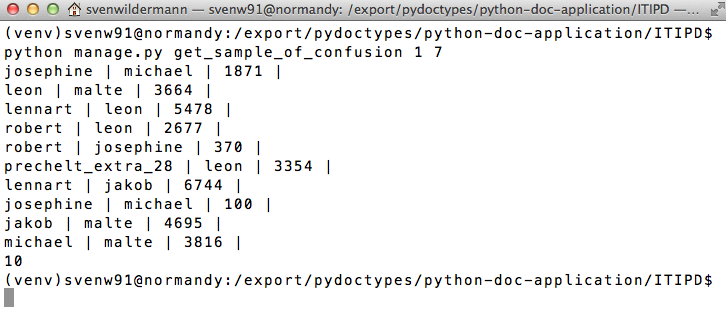
\includegraphics[width=1.0\textwidth]{pictures/terminal-confusion-sample.png}
\caption[Funktion f�r die Konfusions-Stichprobe]{Funktion f�r die Konfusions-Stichprobe}
\label{fig:Funktion-Konfusion}
\end{figure}

\subsection{Ergebnis-Zusammenf�hrung der Goldstichproben}
Da die Goldstichprobe insgesamt drei mal von verschiedenen Gutachtern typisiert wurde, m�ssen diese f�r die weitere Verwendung zusammengef�hrt werden. Um aus drei Wahrheiten die "`eine"' zu machen, wird wie folgt vorgegangen: \\
Es werden alle m�glichen Tupel auf die Gesamtvertr�glichkeit �ber alle Zeichen berechnet . Zwei dieser drei Tupel besitzen somit automatisch den selben Gutachter, so dass diese damit die h�chste Gesamtvertr�glichkeit f�r diese Einheit besitzt. Die Markierungen dieses Gutachtern werden dann einem "`Dummy-Benutzer"' kopiert. \\
Anschlie�end werden die Markierungen der Gutachter mit dem des Dummys manuell verglichen und wo n�tig noch kleinere Korrekturen vorgenommen. 
Diese sind vor allem folgender Natur:
\begin{itemize}
\item Es gibt eine Markierung, die die anderen zwei Gutachter get�tigt haben (also nicht in den Markeriungen des Dummys vorkommt). Daher wird eine Markierung des Dummys durch die der anderen Gutachter ersetzt oder hinzugef�gt (je nach �bereinstimmung der Segementierungen).
% Beispiel mit Screenshots!? 
\item Mindestens einer der Gutachter hat richtig ein Segement mit dem Wissenstyp "`Strucutre and Relationship"' markiert. Wenn dieses in der aktuellen Fassung des Dummys fehlt, wird es hinzugef�gt.
\item Mindestens einer der Gutachter hat richtig ein Segement mit dem Wissenstyp "`External References"' markiert. Wenn dieses in der aktuellen Fassung des Dummys fehlt, wird es hinzugef�gt. 
\end{itemize}
Somit erh�lt man ein endg�ltiges, fast ideales Ergebnis der Goldstichprobe. Ein �hnlicher Vorgang muss jetzt mit der Hauptstichprobe geschehen.

% Es wurden nicht die Markierungen direkt �berpr�ft und �bernommen, da ansonsten mehr Markierungen als �blich �bernommen worden w�ren !?!? 

\subsection{Ergebnis-Zusammenf�hrung der Hauptstichproben}
Da jede Einheit aus der Hauptstichprobe ebenfalls von zwei Gutachtern bewertet wurde, m�ssen auch diese Ergebnisse zusammengef�hrt werden. 
Diese Stichprobe ist mit 1548 Einheiten allerdings erheblich gr��er als die Goldstichprobe mit 168 Einheiten, deswegen soll dies durch ein Skript (Django-Kommando) automatisiert werden. 

\subsubsection{Markierungsresultat bestimmen} 
\label{par:Markierungsresultat}
Das Markierungsresultat wird f�r die Markierungen der Gutachter $G_{i}$ und $ G_{j}$ wie folgt bestimmt: \\
Die Markierung werden nach ihrem Auftreten aufsteigend sortiert. 
Nacheinander werden alle Markierungen, die sich zu mindestens 50 Prozent �berschneiden, mit einander verglichen. Sobald ein Gutachter bei diesem Vergleich die Markierung mit dem "`besseren"' Wissenstyp (laut Konfusionergebnis) get�tigt hat, bekommt dieser einen "`Pluspunkt"' und seine Markierung wird in das Endresultat �bernommen. Wenn es f�r eine Markierung entweder eine �bereinstimmung der Wissenstypen gibt oder diese so verschieden sind, dass diese nicht zu den aufgel�sten Konfusionspaaren geh�ren, dann wird (1) die Markierung des Gutachtern mit mehr "`Pluspunkten"' �bernommen. 
Falls die "`Pluspunkte"' kein eindeutiges Ergebnis liefern, werden die Gutachter mit den besseren Ergebnissen im Vergleich zur Goldstichprobe bevorzugt. 


\subsection{Auswertung der Typisierungen}

\subsubsection{�bereinstimmung pro Wissenstyp nach Gutachtern}
Die �bereinstimmung der Wissenstypen nach Gutachtern wurde in der vorangegangen Studie wie folgt gemessen \cite{MaalejRobillard}:
\begin{shaded}
"`We calculated the agreement score for $C_{i} $by dividing the number of ratings which agree with the second coder by the total number of units coded by $C_{i}$. For example, if $C_{i}$coded 500 units and 400 of their Functionality ratings were the same as the ratings of the co-coder, $C_{i} $s agreement score for Functionality would be $400/500 = 0.80$. We calculated the overall agreement by summing all agreements over all variables and dividing by the number of units times 12 (the number of variables)."' 
\end{shaded}
Diese Auswertung habe ich analog auf diese Arbeit �bertragen und mittels eines Django-Kommandos umgesetzt. 
Ein Wissenstyp in einer Einheit ist vorhanden, sobald mindestens eine Markierung mit diesem in dieser Einheit gefunden wurde. 
Die Konfusionen habe ich dabei nicht aufgel�st, um die Vergleichbarkeit mit der Originalstudie zu erhalten. 
Abbildung \ref{fig:Uebereinstimmung_Gutachtern} zeigt die �bereinstimmung nach Gutachtern. Die ersten drei Spalten geben den kleinsten, den durchschnittlichen und den gr��ten Wert aller Gutachter f�r einen Wissenstypen an. Die letzten beiden Spalten identifizieren die Gutachter mit der besten und der schlechtesten �bereinstimmung. Der durschnittliche Wert ist dabei �ber alle Wissenstypen hinweg gr��er als 0,75 und insgesamt gr��er als 0,87. 

\begin{figure}[H]
\begin{tabular}{c c c c c c} \hline
\textbf{Wissenstyp} & \textbf{Min} & \textbf{Durschn.} & \textbf{Max.} & \textbf{Bester} & \textbf{Schlechtester}  \\ \hline
Functionality & 0,730 & 0,786 & 0,926 & C9 & C6 \\
\rowcolor{gray!20 }Concepts& 0,792 &0,855 & 0,963 & C9 & C5 \\
Directives& 0.803 & 0,876 & 0,929 & C8 & C6 \\
\rowcolor{gray!20 }Purpose& 0,703 & 0,788 & 0,857 & C8 & C6 \\
Quality&0,820 & 0,863 & 0,910 & C1 & C4 \\
\rowcolor{gray!20 }Control-Flow&0,893 & 0,943 & 0,964 & C6 & C8 \\
Structure&0,633 & 0,751 & 0,817 & C5 & C4 \\
\rowcolor{gray!20 }Patterns&0,873 & 0,903 & 0,964 & C8 & C5 \\
Code-Examples&0,963 & 0,984 & 1,0 & C8 & C9 \\
\rowcolor{gray!20 }Environment&0,890 & 0,950 & 1,0 & C8, C9 & C6 \\
References&0,951 & 0,969 & 0,977 & C4 & C2 \\
\rowcolor{gray!20 }Non-Info&0,765&0,857 & 1,0 & C8 & C4 \\ \hline
\textbf{Gesamt} & 0,818 & 0,877 & 0,942 & C8 & C6 \\ \hline
\end{tabular}
\caption{�bereinstimmung nach Gutachtern}
\label{fig:Uebereinstimmung_Gutachtern}
\end{figure}

%\paragraph{Ergebnis}
%\paragraph{Vergleich zum Originalartikel}
%\paragraph{Detailierte Auswertung}


\subsubsection{�bereinstimmung nach Wissenstyp}
Die �bereinstimmung nach Wissenstypen wurde in der Studie von Maalej und Robillard wie folgt berechnet \cite{MaalejRobillard}:
\begin{shaded}
"`We measure agreement for a variable by dividing the number of units for which the two coders agreed (i.e., both rated True or both rated False) over the total number of units. This measure of raw agreement is one among many alternatives for measuring agreement by variable [25]. The advantage of the raw agreement measure is that it is simple to interpret. The disadvantage is that it does not take into account that coders might agree by chance."'
\end{shaded}
Auf Grund der ver�nderten Typisierungweise in dieser Arbeit ist eine �bereinstimmung durch Zufall sehr viel unwahrscheinlicher, weshalb diese Auswertung f�r diese Arbeit eher uninteressant ist und somit nicht durchgef�hrt wird.  
% ganz weglassen? 

\subsubsection{�bereinstimmung nach Einheiten}
Zus�tzlich kann die �bereinstimmung nach Einheiten berechnet werden. 
F�r jede Einheit wird f�r jeden Wissenstyp gepr�ft, ob die Gutachter mindstens eine Markierung dieser Art get�tigt haben. 
Eine �bereinstimmung liegt dann vor, wenn bei beide Gutachter sich einig sind, ob dieser Wissenstyp (mindestens einmal) vorkommt oder nicht. Da es insgesamt 12 Wissenstypen gibt, entspricht jede �bereinstimmung in einem Wissenstyp $\frac{1}{12} = 8,33\%$ . F�r jeden Gutachter wird so die �bereinstimmung �ber alle Einheiten berechnet und der Durchschnittswert in Abbildung \ref{fig:Uebereinstimmung_Einheit} ausgegeben. Der Zeile f�r des besten Gutachtern ist gr�n, die des schlechtesten ist rot markiert. Analog wird der Durchschnittswert f�r die unterschiedlichen Kategorien in Abbildung \ref{fig:Uebereinstimmung_Einheit_Kategorie} angezeigt. \\
Diese �bereinstimmung pr�ft somit nicht nur, ob sich zwei Gutachter darin einig sind, dass ein Wissenstyp vorhanden ist, sondern auch, ob sie sich darin einig sind, dass dieser nicht vorhanden ist. 

\begin{figure}[H]
\centering
\begin{tabular}{|c|c|} 
Gutachter & �bereinstimmung \\ \hline
\rowcolor{gray!20}C1 & 0,873 \\
C2 & 0,882\\
\rowcolor{gray!20 }C3 & 0,855\\
C4 & 0,848\\
\rowcolor{gray!20 }C5 & 0,870\\
\rowcolor{red!20 }C6 & 0,845\\
\rowcolor{gray!20 }C7 & 0,882\\
C8 & 0,898\\
\rowcolor{green!20 }C9 & 0,907\\ \hline
\textbf{Durchsch.} & 0.866 \\ 
\end{tabular}
\caption{�bereinstimmung nach Einheit je Gutachter}
\label{fig:Uebereinstimmung_Einheit}
\end{figure}

\begin{figure}[H]
\centering
\begin{tabular}{|c|c|}
Kategorie & �bereinstimmung \\ \hline
\rowcolor{gray!20 }Methoden & 0,845 \\
Felder & 0,876 \\
\rowcolor{gray!20 }Module & 0,805 \\
Klassen & 0,839 \\
\rowcolor{gray!20 }Beschreibungen & 0,916 \\
% man erkennt deutlich: Je l�nger eine Einheit (siehe Durchschnitt) desto schwieriger ist die gleiche Bewertung dieser Einheit
\end{tabular}
\caption{�bereinstimmung nach Einheit je Kategorie}
\label{fig:Uebereinstimmung_Einheit_Kategorie}
\end{figure}
\subsubsection{Rechenbeispiel}
Um die Bedeutung dieser Berechnungen zur �bereinstimmung zu veranschaulichen, folgt ein Beispiel: \\
Eine Einheit wird von beiden Gutachtern mit genau einem Wissenstypen markiert. Gutachter A vergibt den Wissenstyp 1 und Gutachter B vergibt den Wissenstyp 2. Somit sind sich Gutachter A und B dar�ber einig, dass die anderen zehn Wissenstypen (drei bis zw�lf) nicht vorhanden sind. Dies ergibt eine �bereinstimmung in dieser Einheit von $\frac{10}{12} = 83,33 \% $. \\
Die �bereinstimmung misst somit nicht nur die Einigkeit �ber das Vorhandensein eines Wissenstypen sondern auch �ber das Fehlen dessen. 
\subsubsection{�bereinstimmung mit Goldstichprobe}
Um die Gutachter entsprechend der Qualit�t ihrer Leistungen einordnen zu k�nnen, werden die Typisierungen dieser mit den Ergebnissen aus der Goldstichprobe verglichen. Aus den �bereinstimmungswerten ergibt sich dann direkt eine Platzierung f�r jeden Gutachter. Die �bereinstimmung wird analog zu der in Kapitel XY berechnet. 

%***START***
%username:robert
%75.36790099999999
%20
%***********
%username:jakob
%85.37473274509804
%51
%***********
%username:josephine
%71.56433599999998
%60
%***********
%username:lennart
%80.06050749999999
%48
%***********
%username:leon
%74.98821765957446
%47
%***********
%username:malte
%65.16846339285715
%56
%***********
%username:michael
%81.51374388888888
%54
%***********
%username:prechelt_extra_28
%could not compare anything
%***********
%username:sven_extra_28
%could not compare anything
%***********


%***START***
%username:robert
%90.536611
%20
%***********
%username:jakob
%93.37414372549017
%51
%***********
%username:josephine
%90.58970899999998
%60
%***********
%username:lennart
%93.78278312500002
%48
%***********
%username:leon
%91.21594531914893
%47
%***********
%username:malte
%89.75318660714287
%56
%***********
%username:michael
%96.26911648148149
%54
%***********
%username:prechelt_extra_28
%could not compare anything
%***********
%username:sven_extra_28
%could not compare anything
%***********



\subsubsection{Unstimmigkeiten zur Goldstichprobe}
Solange sich zwei Gutachter einig sind, wird das Ergebnis der Markierungen als g�ltiges Endresultat anerkannt. Wenn jedoch zwei Gutachter den falschen Wissenstypen w�hlen, zum Beispiel weil sie beide den Wissenstypen X mit Wissenstyp Y verwechseln, wird dieses Ergebnis verf�lscht. Um solche Tendenzen der Gutachter aufzeigen zu k�nnen, vergleiche ich die gefundenen Wissenstypen (als zw�lf boolsche Werte) der Gutachter mit den Ergebnissen aus der Goldstichprobe. Dabei gibt es zwei unterschiedliche Unstimmigkeiten:
\begin{enumerate}
\item Falsch-Positiv: Gutachter gibt an, dass der Wissenstyp in dieser Einheit vorhanden ist, obwohl dies laut Goldstichprobe nicht der Fall ist.
\item Falsch-Negativ: Gutachter hat keine Markierung mit diesem Wissenstyp get�tigt, obwohl in der Goldstichprobe mindestens eine davon vorhanden ist. 
\end{enumerate}
Im folgenden wird f�r jeden Wissenstyp dargelegt, wie oft die Gutachter die Einheiten der Goldstichprobe falsch markiert haben sowie welche Anteile durch die falsch-positiv (FP) und falsch-negativen (FN)  Bewertungen verursacht wurden. Da jede Einheit doppelt typisiert wurde, liegt eine Menge von 336 Typisierungen mit insgesamt $336 * 12 =  4032$\footnote{Es gibt 12 Wissenstypen} Bewertungen zu Grunde. 
\begin{figure}[H]
\centering
\begin{tabular}{|c|c|c|c|c|} \hline
\textbf{Wissenstyp} & \textbf{Gesamt} & \textbf{FP} & \textbf{FN}  \\ \hline 
Functionality & 51 & 0,255 & 0,745 \\
\rowcolor{gray!20 }Concepts& 33 &0,667 & 0,333 \\
Directives& 47 & 0,596 & 0,404  \\
\rowcolor{gray!20 }Purpose& 34  & 0,765 & 0,235  \\
Quality& 45 & 0,378 & 0,622  \\
\rowcolor{gray!20 }Control-Flow&17  &  0,412 & 0,588 \\
Structure& 83 & 0,361 & 0,639   \\
\rowcolor{gray!20 }Patterns & 25 & 0,560 & 0,440 \\
Code-Examples &9 & 0,667 & 0,333  \\
\rowcolor{gray!20 }Environment& 16 & 0,625  & 0,375  \\
References& 15 & 0,333  & 0,667 \\
\rowcolor{gray!20 }Non-Info& 40 &0,850 & 0,15 \\ \hline
\textbf{Gesamt} & 415 & 0,539 & 0,461 \\ \hline
\end{tabular}
\end{figure} 

\textbf{HIER NOCH DIE HAUPT-VERURSACHER MIT AUFNEHMEN}


\subsubsection{Vertr�glichkeit von Einheiten}
Weiterhin wird die Vertr�glichkeit der Einheiten betrachtet und ausgewertet. 
Die Vertr�glichkeit bezieht sich auf die einzelnen Markierungen einer Einheit und ist wie folgt definiert. \\
\textbf{Definition:} Eine Markierung ist vertr�glich, wenn es eine andere Markierung gibt, die  
\begin{enumerate}
\item diese umschlie�t (gr��er oder gleich gro� ist) \textbf{oder}
\item zu mindestens 50 Prozent Teil dieser Markierung ist
\end{enumerate}
und beide Markierungen den selben Wissenstypen oder eine Kombination aus den Konfusionspaaren besitzen. \\
Oder anders ausgedr�ckt: \\
Sei $B_{i}$ der Beginn, $E_{i}$ das Ende und $W_{i}$ der Wissenstyp der Markierung i, "`\&' das Zeichen f�r das logische "`und"', "`||"' das Zeichen f�r das logische "`oder"' und $confusion(i,j)$ eine Funktion, die angibt, ob die Wissenstypen i und j zu den aufgel�sten Konfusionen geh�ren. Dann hei�en zwei Markierungen M1 und M2 vertr�glich, wenn:
\begin{enumerate}
\item $(B_{1}>=B_{2}) $ \& $ (E_{1}<=E_{2})$ \textbf{||}
\item $(B_{1}<=E_{1}>=B_{2}) $ \& $ ((E_{1}-B_{2})>=\frac{E_{1}-B_{1}}{2})$
\end{enumerate}
\textbf{\&} $(W_{1} = W_{2}$ \textbf{||} $confusion(W_{1},W_{2}) )$ \\ \\ 
Die Vertr�glichkeiten f�r jede Einheit werden auf zwei Weisen berechnet:
\begin{enumerate}
\item nach Anzahl der Markierungen. Dabei wird die Anzahl der vertr�glichen Markierungen durch die Anzahl der gesamten Markierungen beider Gutachter pro Einheit geteilt.
\item nach der Menge der vertr�glichen Zeichen. Hier wird die Anzahl aller Zeichen von vertr�glichen Markierungen durch die Anzahl aller Zeichen der Markierungen beider Gutachter geteilt.
\end{enumerate}

W�hrend in Abbildung \ref{fig:Vertr�glichkeit_Gutachter} die durchschnittliche Vertr�glichkeit pro Gutachter dargestellt wird, zeigt Abbildung \ref{fig:Vertr�glichkeit_Kategorie} diese pro Kategorie.

% �bersehen von kleinen Segmenten wird bei der zweiten Methode weniger stark ber�cksichtigt -> fairer

\begin{figure}[H]
\centering
\begin{tabular}{|c|c|c|} 
& \multicolumn{2}{c}{Vertr�glichkeit} \\
Gutachter & (1) nach Zeichen & (2) nach Markierungen \\ \hline
\rowcolor{gray!20}C1 & 0,819 & 0,786 \\
C2 & 0,848 & 0,823 \\
\rowcolor{gray!20 }C3 & 0,818 & 0,788\\
C4 & 0,704 & 0,674 \\
\rowcolor{gray!20 }C5 & 0,860 & 0,829 \\
C6 & 0,783 & 0,750 \\
\rowcolor{gray!20 }C7 & 0,841 & 0,809 \\
C8 & 0,922 & 0,895 \\
\rowcolor{gray!20 }C9 & 0,863 & 0,820 \\ \hline
\textbf{Durchsch.} & 0.828 & 0,797  \\ 
\end{tabular}
\caption{Vertr�glichkeit nach Gutachtern}
\label{fig:Vertr�glichkeit_Gutachter}
\end{figure}

\begin{figure}[H]
\centering
\begin{tabular}{|c|c|c|} 
& \multicolumn{2}{c}{Vertr�glichkeit} \\
Kategorie & (1) nach Zeichen & (2) nach Markierungen \\ \hline
\rowcolor{gray!20 }Methoden & 0,879& 0,800\\
Felder &0,725& 0,719 \\
\rowcolor{gray!20 }Module &0,791& 0,730  \\
Klassen &0,721& 0,698 \\
\rowcolor{gray!20 }Beschreibungen &0,861& 0,854 \\
\end{tabular}
\caption{Vertr�glichkeit nach Kategorien}
\label{fig:Vertr�glichkeit_Kategorie}
\end{figure}


\section{Fazit}
Das Ziel dieser Arbeit war das �bertragen der Informationtypen-Analyse von Walid Maalej und Martin Robillard \cite{MaalejRobillard} auf die Python-Dokumentation.
Mit Hilfe der erhobenen Daten und der dar�ber ausgef�hrten Auswertungen k�nnen nun fundierte Aussagen �ber die Art und Verteilung von Informationen in der Dokumentation getroffen werden. Au�erdem k�nnen diese Daten mit den Ergebnissen f�r die Dokumentationen in JAVA und .NET verglichen werden. 
Insgesamt kann die Durchf�hrung dieser Arbeit als Erfolg gewertet werden, da �ber eine reine Folgestudie hinaus noch einige Verbesserungen im Ablauf vorgenommen wurden, die sich auf die Qualit�t der Ergebnisse ausgewirkt haben. 

\subsection{Vergleich}
Es ist zu beachten, dass es teilweise Unterschiede in den Berechnungen dieser Arbeit und der Originalstudie gibt. 
Da in dieser Arbeit die Zuordnung der Wissenstypen nicht �ber das Setzen von Haken in "`CheckBoxes"', sondern �ber das Markieren von Zeichenketten geschieht, sind die Ergebnisse nicht nur detailreicher, sondern auch weniger zuf�llig. Daher entfallen die Auswertungen dar�ber, wie wahrscheinlich es ist, dass sich zwei Gutachter zuf�llig einig sind. 
\\
Dennoch gibt es einige Auswertungen, die sowohl in dieser Arbeit als auch in der anderen Studie vorgenommen wurden. Die Berechnung der �bereinstimmung von Typisierungen verschiedener Gutachter wurde analog ausgef�hrt und zeigt, dass in dieser Arbeit die �bereinstimmungen zwischen den Gutachtern im Median um fast sechs Prozent h�her sind (82 Prozent zu 87,9 Prozent). Die Werte f�r die minimale und die maximale �bereinstimmung zwischen zwei Gutachtern sind sogar fast zehn Prozent h�her. Das f�hrt zu dem Schluss, dass die in dieser Arbeit gew�hlte Methode zur Erfassung von Informationstypen zu gr��erer Sorgfalt gef�hrt hat, obgleich die Dauer f�r die Typisierung pro Einheit anstieg. \\
Die Berechnungen f�r die Unstimmigkeiten zwischen den Gutachtern sind in dieser Arbeit erheblich anders durchgef�hrt worden als in der Originalstudie und bieten somit keine direkte Vergleichsm�glichkeit. Man erkennt aber sehr wohl, dass es bei beiden Studien nur wenige Unstimmigkeiten bez�glich des Wissenstypen "`Code Examples"' gibt und eher viel Uneinigkeit dar�ber, wann die Wissenstypen "`Structure and Relationship"' und "'Functionality and Behaivor"' zutreffend sind. \\
Die Verteilung der verschiedenen Wissenstypen �ber alle Einheiten zeigt einige Parallelen. So sind allen drei Dokumentationen (Java, .NET, Python) viele Einheiten mit dem Wissenstyp "`Functionality and Behavior"' vorhanden.  Zu etwa 20 Prozent kommt in allen untersuchten Dokumentationseinheiten auch der Wissenstyp "`Structure and Relationship"' vor. Einen entscheidenden Unterschied gibt es bei der Menge an Einheiten mit dem Wissenstyp "`Non-Information"'. W�hrend bei Java und .NET in etwa der H�lfte der Dokumentationseinheiten dieser Typ identifiziert wurde, waren es bei Python nur etwa sechs Prozent. \\
Wenn man die nach Kategorie aufgeteilten Wissenstypen beider Studien vergleicht, erkennt man bei Java und Python denselben Wert f�r die Kategorie "`Klassen"' und den Wissenstyp "`Functionality and Behaivor"'. In beiden Dokumentationen liegt der Wert bei 64 Prozent. Fast identisch sind zudem die Werte dieser Kategorie f�r die Typen "`Structure and Relationship"' und "`Directives"'. Gleichzeitig findet man in etwa jeder zweiten Methodenbeschreibung in JAVA und .NET "`Non-Information"'. Bei Python ist dies gerade einmal in jeder f�nfzigsten Methode der Fall. \\
Analog zur Originalstudie wurde auch in dieser Arbeit eine starke Korrelation der Typen "`Patterns"' und "`Examples"' gefunden. �berlagert man die Grafiken, sind �hnliche Muster erkennbar. Dazu geh�ren beispielsweise die geringe positive Korrelation der Typen "`Non-Information"' und "`References"' zu allen anderen Wissenstypen sowie die hohe Korrelation der Wissenstypen "`Examples"' und "`Patterns"' zu allen �brigen Wissenstypen.\\
Der proportionale Zusammenhang zwischen der Anzahl der W�rter in einer Dokumentationseinheit und der Anzahl der Wissenstypen konnte in der vorangegangen Studie ebenso gezeigt werden wie in der vorliegenden. Dabei fiel das Ausma� des Zusammenhangs bei der Python-Dokumentation �ber alle Kategorien hinweg deutlicher aus, als es bei Java und .NET der Fall war. Gleichzeitig ist zu bemerken, dass der Plaintext\footnote{Technischnische Bezeichnung f�r Klartext} in dieser Arbeit mit Hilfe des in BeautifulSoup definierten Befehls 
\begin{lstlisting}
	findAll(text=True)
\end{lstlisting}
bereits im Extrahierer ausfindig gemacht wurde und dieser so m�glicherweise mehr (Leer-)zeichen enth�lt als angezeigt werden. Daher werden unter Umst�nden auch mehr als die sichtbaren W�rter gez�hlt. Die �berpr�fung dieses Verdachts bedarf einer weiteren Datenanalyse. \\
Zusammengefasst konnten sowohl wichtige Gemeinsamkeiten als auch Unterschiede zwischen den Dokumentationen von Java, .NET und Python gefunden werden. 
Vor allem der viel geringe Anteil an Nicht-Information bei gleichzeitig h�herem Anteil an "`Functionality and Behavior"'-Wissenstypen in der Python-Dokumentation kann als Vorteil dieser gegen�ber den anderen gewertet werden. 

\subsection{Ausblick}
Mit den erhobenen Daten k�nnen �ber diese Bachelorarbeit hinaus noch viele andere Auswertungen get�tigt werden. Beispielsweise kann untersucht werden, welche Markierungen sich in der Regel �berlappen und in welcher Syntax dies geschieht. Damit erh�lt man dann eine Aussage dar�ber, welche Informationstypen zusammen in einem Satzgebilde verf�gbar sind. \\
Weiterhin kann betrachtet werden, in welcher Reihenfolge bestimmte Wissenstypen auftauchen. Das ist ein wichtiger Schritt, um die Semantik hinter der Syntax zu verstehen. Man kann beispielsweise durch die Korrelation von "`Examples"' und "`Pattern"' davon ausgehen, dass in der Regel erst "`Pattern"' (wie setze ich XY um) beschrieben wird und im Anschluss daran ein Programmierbeispiel folgt. Diese Vermutungen k�nnen dann durch Analysen best�tigt oder widerlegt werden. \\
Die Menge der Information je Informationstyp kann durch die vorliegenden Daten sehr genau analysiert werden. W�hrend in der Originalstudie von Walid Maalej und Martin Robillard bekannt wird, ob ein Wissenstyp vorhanden ist, kann man jetzt sogar aussagen, wie viel davon vorhanden ist. Bei den �bereinstimmungswerten ist diese Analyse zu Teilen bereits mit eingeflossen. \\
Um die bis hierhin genannten Auswertungen in Relation zu anderen Dokumentationen auswerten zu k�nnen, sollte diese Art der Auswertung auch mit JAVA und .NET-Dokumentationen (und weiteren) wiederholt werden. Nur so kann langfristig der objekte Unterschied zwischen den Dokumentationen g�nzlich verstanden werden. 
\\  \\
Sofern weitere Analysen bez�glich Dokumentationen f�r Programmiersprachen folgen, kann m�glicherweise schon bald auf Grundlage dieser ein Leitfaden f�r gute Dokumentationen ver�ffentlicht werden. Ziel dieses sollte es dann sein, den Informationsgehalt der Dokumentationen m�glichst zu steigern und geringwertige Informationen zu vermeiden. Schlie�lich kann Programmcode nur so gut sein wie das Verst�ndnis des Programmierers und dieses wiederum nur so gut wie die vorliegenden Informationen zu der Programmiersprache. 

%\newpage
%\thispagestyle{empty}
%\mbox{}
%\newpage
\section{Anhang}
\subsection{Quelltext}
Die entwickelten Werkzeuge (Website, Extrahierer, Django-Kommandos) stehen als GIT-Repository auf bitbucket.org zur Verf�gung:\\
\href{https://bitbucket.org/svenwildermann/python-doc-application}{https://bitbucket.org/svenwildermann/python-doc-application}. \\
Der letzte Commit\footnote{Befehl des Versionskontrollsystems "`GIT"' f�r das Bekanntgeben von �nderungen} fand am 9. August 2014 statt und besitzt folgenden HASH-Wert, wobei die ersten sieben Zeichen bereits f�r eine Identifizierung gen�gen:
\begin{lstlisting}
34cbc4765d485f3d76cc33e89622b5509bc026bc
\end{lstlisting}
Die Angabe dieses Wertes best�tigt den Stand der Programmierung zum Zeitpunkt der Abgabe. Weiterentwicklungen nach Abgabe der Bachelorarbeit sind, speziell f�r weiterf�hrende Auswertungen �ber den Rahmen dieser Arbeit hinaus, m�glich und ggf. auch n�tig. 


%\subsection{Kodierhandbuch, vollst�ndig}
%Dieser Abschnitt enth�lt das vollst�ndige Kodierhandbuch \cite{codingguide_new} , welches f�r die Gutachter zur Verf�gung gestellt wurde. Zeitpunkt der Kopie: 6. August 2014.  
%
%\begin{shaded}
%\section*{Knowledge Types}

\subsection*{1 Functionality and Behavior}
Describes what the API does (or does not do) in terms of functionality or features. The block describes what happens when the API is used (a field value is set, or a method is called). This also includes specified behavior such as what an element does, given special input values (for example, null). \\

Functionality and behavior knowledge can also be found in the description of parameters (e.g., what the element does in response to a specific input), return values (e.g., what the API element returns), and thrown exceptions.
\\
Detects stream close and notifies the watcher
Obtains the SSL session of the underlying connection, if any. If this connection is open, and the underlying socket is an SSLSocket, the SSL session of that socket is obtained. This is a potentially blocking operation.
Only rate this type as true if the block contains information that actually adds to what is obvious given the complete signature of the API element associated with the block. If a description of functionality only repeats the name of the method or field, it does not contain this type of knowledge and you should rate it as false, and instead rate the knowledge type non-information as true. For example, this would be the case if the documentation for a method called getTitle was
\\
Returns the title.
Similarly for constructors, if the documentation simply states "Constructs a new X", "Instantiates a new object", or something similar the value is false (with non-information coded as true). In some cases non-information will be phrased to look like a description of functionality, for examples with sentences that start with verbs like "gets", "adds", "determines", "initializes". Carefully read the name and signature of the API element and only assign a value of true for this knowledge type if the block adds something to the description of the element.

However, if any other details are provided, rate this type as true. For example:

Creates a new MalformedChallengeException with a null detail message.
Should get a value of true because of the additional information about the value of the message field.

Mentioning that a value can be obtained from a field, property, or getter method does not constitute a description of functionality, except the API performs some additional functions when the value is accessed. For example, the block below does not represent a description of functionality. The Non-information type for this block should be rated as true.

[LoggerDescription.Verbosity Property] Gets the verbosity level for the logger.
Note IMPORTANT: Description of functionality is not limited to the functionality of the element associated with the block, but the API as a whole. However, if the block explains a sequence of method calls or creation of particular objects (e.g. events) code this as Control-Flow. For example, if setting the value of a field results in some perceived behavior by the framework, this knowledge counts as functionality. If the block describes a resulting sequence of method calls or events fired, this is control flow. If the block contains both, then both should be coded as true.

2 Concepts

Explains the meaning of terms used to name or describe an API element, or describes a design or domain concepts used or implemented by the API. Code this knowledge type with a value of true if an explanation of concepts is provided, with some useful details. The sentences below show an example of a description of the concept of "secure sockets".

Plain sockets may be considered secure, for example if they are connected to a known host in the same network segment. On the other hand, SSL sockets may be considered insecure, for example depending on the chosen cipher suite.
Note: Basic description of the parameters does not represent concept description, such as

header - the challenge header [in a method called processChallenge]
In this case, the knowledge type Non-Information should be set to true.

3 Directives

Specifies what users are allowed / not allowed to do with the API element, in particular any caller-created condition that will raise an exception. Directives are clear contracts. For example how callers must deal with return values, what is permitted by implementers of abstract elements, limitations on the sequences in which API elements may be accessed, or any explicit mention of the input values that are allowed (or not allowed) for an API element (e.g. parameters values for methods or values that can be assigned to fields).

In Python, mentioning the required type of a parameter (as opposed to other constraints on the parameter value) is not considered a directive, unless a forbidden type is mentioned explicitly or the term "must"/"has to" etc is used.

If this method returns false, the caller MUST close the connection to correctly comply with the HTTP protocol. If it returns true, the caller SHOULD attempt to keep the connection open for reuse with another request.
An implementation is free to throw an exception, deliver a null result, deliver a misleading value, whatever is convenient.
[Clients] should ensure that the resulting list is asserted back into the graph into the appropriate relationships
Instances of this class are unmodifiable
An index between 0 and 100.
This parameter can be true, false or ?default? (null).
In contrast to Patterns, directives represent specific contracts or constraints on how to use a specific element and the API.

4 Purpose and Rationale

Explains the purpose of providing an element or the rationale of a certain design decision. Typically, this is information that answers a "why" question: Why is this element provided by the API? Why is it this designed this way? Why would we want to use this? This includes in which context an API element can (or should) be used, or the advantages of using the element.

This allows for the header to be sent without another formatting step.
This is important for generating the Cookie header because some cookie specifications require that the Cookie header should include certain attributes only if they were specified in the Set-Cookie header.
[If EOF is detected, the watcher will be notified and this stream is detached from the underlying stream.] This prevents multiple notifications from this stream.
This method can be used for obtaining metainformation about the entity implied by the request without transferring the entity- body itself.
It can be used to quickly parse large amounts of text to find specific character patterns
This enables the programmer to write code in a compact and easy style.
Note: Descriptions of cases, where an element (such as a field) is used by the API, fall under either Functionality or Control-Flow, as appropriate. Note also that sometimes the difference between purpose and functionality can be confused. For example, for a method drawCircle(int r) the description "draws a circle of radius r" could be interpreted as "the purpose is to draw a circle", or "this method should be used to draw a circle". For this study this is not the correct interpretation. Only code a value of true for purpose if the block contains a description of the purpose that is not self-evident from the method"s functionality.

5 Quality Attributes and Internal Aspects

Describes quality attributes of the API, also known as non-functional requirements, for example, the performance or security implications of using the API element (or related elements), such as resources consumed or the execution time of a method. Also code with a value of true if the block provides information about API"s internal implementation that is only indirectly related to its observable behavior. For example, indicates the main data structures and algorithms employed.

This is a ?graceful? release and may cause IO operations for consuming the remainder of a response entity.
Enumerating through a collection is intrinsically not a thread-safe procedure.
6 Control-Flow

Describes how the API (or the framework) manages the flow of control, for example by stating what events cause a certain callback to be triggered, or by listing the order in which API methods will be automatically called by the framework itself. Wherever you find a clear description of the sequence of methods that result in calling an API, code control-flow knowledge as true (see Functionality).

On the client side, this step [the callback] is performed before the request is sent to the server.
Changing the value of Path for a DirListBox control generates an Change event.
Note: Descriptions of how the programmer should organize the control-flow of their code when using the API do not apply here. Instead, see the knowledge types Patterns, Functionality, or Example.

7 Structure and Relationships

Describes the internal organization of a compound element (for example important classes, fields, or methods), information about type hierarchies, how elements are related to each other, or the static properties of an element. Basically, structural knowledge is knowledge about how different API elements related to each other.

\verb|Node has five subtypes: Node_Blank, Node_Anon, Node_URI, Node_Variable, and Node_ANY.|
Note that the order of arguments here is different from the similar public constructor, as required by Java
public interface CookieSpec. Cookie management specification must define: a) rules of parsing ?Set-Cookie? header; b) rules of validation of parsed cookies; c) formatting of ?Cookie? header; for a given host, port and path of origin chosen cipher suite.
This class is used with the [LINK] GZipStream and [LINK] DeflateStream classes
Note: Pointers to other sections of the reference documentation of the API (element names, hyperlinks, manually-added "see also" references) can also represent structural information if they indicate how elements relate to each other or what their properties are. (For references to elements in other APIs or to other documents, see the variable References.) For example, a note such as the following contains structural knowledge because it indicates another API element similar to the one documented:

\verb|Same as {@link #close close()}.|
Management interface for client connections. [A link to the class managed by the interface]
However, simply adding a link to another part of the API does not automatically provide structural knowledge if it is not also mentioned why or how this element is related, or its role in the structure of the API. For example

See Also: Constant Field Values
See Also: closeExpiredConnections()
The first link simply points to a collection of constant definition: it does not say anything about how API elements are organized; The second link simply indicates the presence of another method that could be of interest to the programmer, it does not indicate how it relates to the current block. Both of these references should not be marked as structural knowledge.

Only evaluate structural information contained in the block: do not evaluate any automatically generated information, such as the structural information contained in the declaration of an element (e.g. extends MyInterface), or generated links such as "specified by". Be careful. Do not consider any information that is directly derived from the element name, declaring elements, or signature.

8 Patterns

Describes how to accomplish specific outcomes with the API, for example, how to implement a certain scenario, how can the behavior of an element be customized, how can the abstract class be implemented, and how some values can be obtained or some objects created.

Usually this is accomplished by using the ?Decorator? pattern where a wrapper entity class is used to decorate the original entity.
Nodes are only constructed by the node factory methods
The following parameters can be used to customize the behavior of this class - [followed by a multi-line description of the customization options offered by each parameter].
Note: This knowledge type is different from Purpose in that it describes how to do things, not why elements should be used. It is also different from Directives in that it provides guidelines and "how tos". In contrast to Directives, patterns information provides general hints on how to achieve various outcomes with the API, not usage rules and constraints.

9 Code Examples

The block provides code examples of how to use and combine elements to implement certain functionality or design outcomes.

The usual execution flow can be demonstrated by the code snippet below: + CODE SNIPPET
keytool -genkey -v -alias ?my client key? -validity 365 -keystore my.keystore
Note: Code example can also be scripts or other machine instructions. They can be found with patterns but sometimes also without. Similarly, patterns can be enhanced with code example, but can also be found without.

10 Environment

The block contains knowledge about various aspects related to the environment in which the API is used, but not the API directly. For example, compatibility issues, differences between API versions, licensing information. For links to other documents use the Reference types instead.

In Python, a phrase such as "Changed in version x.y:" is always classified as environment; the subsequent text may or may not be.

Since HTTP/1.1, connections are re-used by default. Up until HTTP/1.0, connections are not re-used by default.
This is a change from the behavior of Jena 1, which took a parameter closed to compute the closure over transitivity and equivalence of sub-classes.
This package includes code adapted from Xerces 2.6.0, which is marked and is Copyright (c) 1999-2002 The Apache Software Foundation. All rights reserved.
 

11 External References

The block includes any pointer to external documents, either in the form of hyperlinks, tagged "see also" reference, or mentions of other documents (such as standards or manuals). External documents are any documents except pages in the reference documentation of the Framework currently studied (Java or .NET).

In Python, any hyperlink into the Glossary is considered an External Reference.

Digest authentication scheme as defined in RFC2617.
To find the final URI after any redirects have been processed, please see the section entitled HTTP execution context in the HttpClient Tutorial
 

12 Non-Information

Rate this knowledge as true if the block contains any complete sentence of self-contained fragment of text that provides only uninformative boilerplate text. Common examples include restating the name of the API element without adding any detail, or stating the obvious. Another common case is where the information to explain the return value just restates the information in the rest of the block. However, if a single sentence contains both uninformative and informative text, we consider that the uninformative part of the sentence is only context for the informative part, and in this case you should not rate it as non-information.

uri - The URI
IOException - If something happens.
[PanelArray.ControlAdded] Event Occurs when a new control is added to the PanelArray.
Note: Non-Information is not mutually exclusive with Functionality knowledge. If the block only restates the name of a method, rate Functionality as false and Non-information as true. If the block provides a true description of the functionality, but just restates this information for example with the return tag, then rate Functionality as true and Non-information as true. In brief, rate Non-information as true whenever a block contains complete sentences or self-contained text fragments that provides no information.
Note
this is different from providing no text whatsoever (empty block), which you should not consider non-information.
The next example shows a combination of directive (the first sentence) and non-information (the second sentence). Although the first sentence provides a directive (do not use this method in your code), the second sentence is just a re-statement of the method"s name. This block would receive a value of true for both the directive and the non-information types.

[FormatUrl.Execute Method] This API supports the .NET Framework infrastructure and is not intended to be used directly from your code. Executes the FormatUrl task.
 

Information to be Coded

Do not evaluate the name of the method. However, you need to read and understand the name to be able to evaluate the documentation.

Please ignore/do not evaluate the following automatically generated sections and blocks:

Java

@deprecated [just the tag but not the text which might follow]
@immutable [just the tag but not the text which might follow]
Java keyword such as implements, extends, throws, return etc.
since:
specified by [and the text which belongs to it]
overrides [and the text which belongs to it]
DotNet

Inheritance Hierarchy [this might be valuable context information]
\verb|Syntax except C#|
Version Information
Platforms
This sentence in section Thread Safety: [Any public static (Shared in Visual Basic) members of this type are thread safe. Any instance members are not guaranteed to be thread safe.]
This sentences in section .NET Framework Security: [Full trust for the immediate caller. This member cannot be used by partially trusted code. For more information, see Using Libraries from Partially Trusted Code.]
References in section See Also that only point to an element"s own class, package/namespace, or to elements directly visible in the declaration of the element associated with the block, such as parameter or return types for a method, declared type for fields.
References in sect See Also without any explanation that relates the reference to the block.
Community Content
Change History
In the code example section, do not take into account the sentence "The Namespace statement must appear outside of any classes or modules." (that is, ignore this sentence, do not count it as a directive or pattern).
 

Tips

Do not interpret too much. Stick to the guide while evaluating knowledge types!
Do not code for more that one hour at once!
Only code as true if the knowledge is clear based on the description of the guide!
Read the guide from time to time!
Do not make too long breaks (e.g. several weeks)!
You might encounter more that one knowledge type in a single sentence.
%\end{shaded}
%\subsection{Technologien}
%In diesem Abschnitt werde ich kurz auf die verwendeten Technologien eingehen und den Einsatz erl�utern. 
%\subsubsection{Django}
%Django ist ein auf Python basierendes quelloffenes Webframework f�r schnelle, saubere und pragmatische Entwicklung. \footnote{https://www.djangoproject.com/}
%Es folgt dem Model-View-Controller-Schema und liegt unter einer BSD-Lizenz vor. 
%\subsubsection{Python}
%\subsubsection{BeautifulSoup4}
%\subsubsection{Coffeescript}
%\subsubsection{Postgres}
%\subsubsection{Ajax}
%\subsection{Glossar}
%\begin{enumerate}
%\item knowledge type/Informationstypen
%\item API - in Implementierung des Extrahierer
%\item DOM-Element
%\end{enumerate}

      

\bibliographystyle{alpha}
\bibliography{bibliography}



\end{document}
